%%
\documentclass[manuscript,screen,12pt, nonacm]{acmart}
\let\Bbbk\relax % Fix for amssymb clash 
\usepackage{standalone}
\usepackage{vmlmacros}
\AtBeginDocument{%
  \providecommand\BibTeX{{%
    \normalfont B\kern-0.5em{\scshape i\kern-0.25em b}\kern-0.8em\TeX}}}
\usepackage{outlines}
%~\usepackage{natbib}
\setlength{\headheight}{14.0pt}
\setlength{\footskip}{13.3pt}
\citestyle{acmauthoryear}
\begin{document}
\title{An Alternative to Pattern Matching, Inspired by Verse}
\author{Roger Burtonpatel}
\email{roger.burtonpatel@tufts.edu}
\affiliation{%
  \institution{Tufts University}
  \streetaddress{419 Boston Ave}
  \city{Medford}
  \state{Massachusetts}
  \country{USA}
  \postcode{02155}
}
\bibliographystyle{plainnat}
% \renewcommand\refname{}
% ~\setcitestyle{sort&compress}


%~\author{Norman Ramsey}
%~\email{nr@cs.tufts.edu}
%~\affiliation{%
%~\institution{Tufts University}
%~\streetaddress{177 College Ave}
%~\city{Medford}
%~\state{Massachusetts}
%~\country{USA}
%~\postcode{02155}
% }

%~\author{Milod Kazerounian}
%~\email{milod.mazerouniantufts.edu}
%~\affiliation{%
%~\institution{Tufts University}
%~\streetaddress{177 College Ave}
%~\city{Medford}
%~\state{Massachusetts}
%~\country{USA}
%~\postcode{02155}
% }

\renewcommand{\shortauthors}{Burtonpatel}


\documentclass[manuscript,screen 12pt, nonacm]{acmart}
\let\Bbbk\relax % Fix for amssymb clash 
\usepackage{vmlmacros}
% Title included so this document can compile alone
\title{An Alternative to Pattern Matching, Inspired by Verse}

\begin{document}


\begin{abstract}
    Pattern matching % S
    appeals % V
    to functional programmers for its expressiveness and good cost model, 
    but 
    it % S
    fails to express % V
    certain computations without verbosity. Verbosity % S 
    can be reduced % V
    by using extended forms of pattern matching,
    but extensions % (S = the problem)
    are % V
    not standardized, and the most desirable combination of extensions cannot be
    found in any one popular programming language. Alternatively to pattern
    matching, computations can be expressed succinctly by using equations, as
    has been demonstrated by the Verse programming language. But such
    computations may have time and space costs that can be hard to predict. 
    % But Verse's cost model % S-sub
    % is % V-sub
    % a challenge because of backtracking and multiple
    % results. 
    As a compromise, 
    I % S
    ~propose % V
     a 
    new language,~\VMinus, % object 
    which~uses equations in a limited way that makes time and space costs easy
    to predict. 
    % to succinctly express computation while
    % enjoying a friendlier cost model by prohibiting backtracking and multiple
    % results. 
    \VMinus~ % S 
    expresses % V
    computations as succinctly as pattern matching with popular extensions in
    comparative examples, and just like pattern matching, it % S
    can be compiled % V 
    to a decision tree. 
    
    An implementation of~\VMinus and its compiler can be found
    at~\url{https://github.com/rogerburtonpatel/vml}.
    % Question: implied that I've implemented D here, or not? 
    %%%%%%% Old, with "I show":
    % I % S
    % ~show % V
    %  that~\VMinus's equations capture the desirable properties of
    % pattern matching with popular extensions, 
    % and I % S-sub
    % ~also
    %  show % V 
    % that~\VMinus~can be compiled to a decision tree and therefore has
    % the same desirable cost model as pattern matching. Finally, 
    % I % S 
    % ~have % V 
    % implemented~\VMinus in Standard ML, alongside an algorithm for compiling it
    % to a decision tree. 
\end{abstract}

\maketitle

\end{document}

\pagebreak
\tableofcontents
\pagebreak
\documentclass[manuscript,screen 12pt, nonacm]{acmart}
\let\Bbbk\relax % Fix for amssymb clash 
\usepackage{vmlmacros}

\begin{document}

\section{Introduction}
% Subjects: Pattern matching and Equations 

Perhaps the most beloved tool among functional programmers for examining and
deconstructing data is pattern matching. 
% It does so implicitly by matching constructed data
% directly against a number of possible forms.
% Maybe combine? 
Pattern matching is also an established and well-researched topic
\citep{wadler1987views, macqueen1985tree, burton1993pattern, palao1996new,
maranget, bpc}. It is appreciated by programmers and researchers alike for two
main reasons: It enables~\it{implicit} data deconstruction, and it has a
desirable cost model. Specifically (regarding the latter), pattern matching can
be compiled to a~\it{decision tree}, a data structure that enforces linear
runtime performance by guaranteeing no part of the data will be examined more
than once.~\citep{maranget}

However, pattern matching cannot express certain common computations succinctly,
forcing programmers who wish to express these computations to duplicate code,
nest~\it{case} expressions, and create multiple points of truth. To mitigate
this, designers of popular programming languages have introduced~\it{extensions}
to pattern matching (Section~\ref{extensions}). 

Extensions strengthen pattern matching, but they are not standardized, so each
popular programming language with pattern matching features its own unique suite
of extensions. Extensions are subject to the discretion of the individual
language designer, not ubiquitous. Rather than continuing to extend pattern
matching~\it{ad hoc}, a worthwhile goal could be to find an alternative that
doesn't need extensions. A tempting possibility was introduced last year by the
programming language Verse~\citep{verse}. In Verse, a programmer can deconstruct
data using a different tool the language offers:~\it{equations}. Equations are
expressive and flexible, and it appears that they can express everything that
pattern matching can, including with popular extensions. 

But a full implementation of Verse is complicated, cost-wise. Verse is a
functional logic programming language, and expressions can backtrack at runtime
and return multiple results, both of which are hard to predict in their costs. 

% A worthwhile goal could be to harmonize the expressive quality of Verse's
% equations with the decision tree property of patterns.

\bf{In this thesis, I~show} that the expressive quality of Verse's equations and
the decision-tree property of patterns can be combined in a single language.
Since the language is a streamlined adaptation of Verse with a reduced feature
set, I~call it~\VMinus (“V minus”). 
% I~also show that~\VMinus subsumes pattern matching with popular extensions. 

To support this claim, I~have formalized~\VMinus with a big-step operational
semantics (Section~\ref{vminus}), I~have formalized decision trees into a core
language~\D (“D”) with a big-step operational semantics (Section~\ref{d}), 
% I~have formalized pattern matching in a core language~\PPlus (“P plus”) with a
% big-step operational semantics (Section~\ref{pplus}),
I~have formalized a translation from~\VMinus to~\D (Sections~\ref{vminustod}),
and I~have implemented both languages in Standard ML. 

\end{document}
\documentclass[manuscript,screen,review, 12pt, nonacm]{acmart}
\let\Bbbk\relax % Fix for amssymb clash 
\usepackage{vmlmacros}
\AtBeginDocument{%
  \providecommand\BibTeX{{%
    \normalfont B\kern-0.5em{\scshape i\kern-0.25em b}\kern-0.8em\TeX}}}
\usepackage{outlines}
\setlength{\headheight}{14.0pt}
\setlength{\footskip}{13.3pt}
\title{An Alternative to Pattern Matching, Inspired by Verse}
\author{Roger Burtonpatel}
\email{roger.burtonpatel@tufts.edu}
\affiliation{%
  \institution{Tufts University}
  \streetaddress{419 Boston Ave}
  \city{Medford}
  \state{Massachusetts}
  \country{USA}
  \postcode{02155}
}
\begin{document}



\section{Pattern Matching and its Extensions}
\label{pmandextensions}

In this section, I~expand on the definitions, forms, and tradeoffs of pattern
matching and equations. These tradeoffs inform the compromises I~make in
\VMinus (Section~\ref{vminus}).


% \1 What is pattern matching 

Pattern matching lets programmers examine and deconstruct data by matching them
against patterns. When a pattern $p$ matches with a value $v$, it can produce
bindings for sub-values of $v$. For example, pattern $x::xs$ matches any 
application of the value constructor \it{cons} (\it{::}), and it binds the first 
element of the cons cell to $x$ and the second to $xs$. 

Why use pattern matching? What could programmers use instead? Before pattern
matching was invented, a programmer had to deconstruct data using \it{observers}
\citep{liskov:abstraction}: functions that explicitly examine a piece of data
and extract its components. Examples of observers in functional programming
languages include Scheme's \tt{null?}, \tt{car}, and \tt{cdr}, and ML's
\tt{null}, \tt{hd}, and \tt{tl}. Given the option of pattern matching, however,
many functional programmers favor it over observers. I~demonstrate with an
example and a claim. 

Consider a \tt{standard\_shape} datatype in Standard ML, which represents shapes
by their dimensions\footnote{For sake of simplicity, \tt{standard\_shape}s
always have an area that can be obtained by standard area formulas: $\frac{1}{2}
* base * height$ for triangles; $\frac{1}{2} * (base_{1} + base_{2}) * height$
for trapezoids.}: 

\medskip 
\begin{minipage}[t]{\textwidth}
    \begin{verbatim}
        datatype standard_shape = SQUARE    of real 
                                | TRIANGLE  of real * real 
                                | TRAPEZOID of real * real * real
\end{verbatim}
\end{minipage}
\medskip 

I~define an \tt{area} function on \it{standard\_shape}s, with this type and these
algebraic laws: 

\medskip 
\begin{minipage}[t]{\textwidth}
    \begin{verbatim}
        area : standard_shape -> real 
           area (SQUARE s)              == s * s 
           area (TRIANGLE (w, h))       == 0.5 * w * h
           area (TRAPEZOID (b1, b2, h)) == 0.5 * (b1 + b2) * h
        
\end{verbatim}
\end{minipage}
\medskip 

Now compare two implementations of \tt{area}, one with observers and one with
pattern matching (Figure~\ref{fig:area}).

    \begin{figure}[H]
      \begin{minipage}[t]{0.7\textwidth}
        \begin{verbatim}
fun observers_area sh =
  if isSquare sh
  then sqSide sh * sqSide sh
  else if isTriangle sh 
  then 0.5 * triW sh * triH sh
  else 0.5 * traB1 sh * traB2 sh * traH sh
            \end{verbatim}
            \Description{An implementation of area observers}
        \subcaption{\tt{area} with observers}
            \label{fig:observersarea} 
      \end{minipage}
      \vfill
      \begin{minipage}[t]{0.7\textwidth}
        % \centering 
        \begin{verbatim}
fun pm_area sh =
  case sh 
    of SQUARE s              => s * s
     | TRIANGLE (w, h)       => 0.5 * w * h
     | TRAPEZOID (b1, b2, h) => 0.5 * (b1 + b2) * h
                \end{verbatim}
       \Description{An implementation of area using implicit deconstruction via
       patterns.}
       \vspace{2.2em}
       \subcaption{\tt{area} with pattern matching}
       \label{fig:pmarea}
      \end{minipage}
      \caption{Implementing \tt{area} using observers is tedious, and the code
      doesn't look like the algebraic laws. Using pattern matching makes an
      equivalent implementation more appealing.}
      \label{fig:area}
    \end{figure}

    Implementing the observers \tt{isSquare}, \tt{isTriangle}, \tt{sqSide},
    \tt{triW}, \tt{traB1}, \tt{traB2}, and \tt{traH} is left as an
    (excruciating) exercise to the reader. 

    In general, pattern matching is preferred over observers for five reasons. 

    \begin{enumerate}
      \item [\textbf{A.}]
      \begin{enumerate}[label=\arabic*]
        \item  \it{Lawlike.} With pattern matching, code more closely
        resembles algebraic laws. 
        \label{p1}
        \item \it{Single copy} With pattern matching, it's easier to avoid
        duplicating code.
        \label{p2}
        \item \it{Exhaustiveness.} With pattern matching, a programmer can
        easily tell if they've covered all cases, and a compiler can verify this
        through \it{exhaustiveness analysis}.
        \label{p5}
    \end{enumerate}

    \item [\textbf{B.}]
    \begin{enumerate}[start=4, label=\arabic*]
      \item \it{Call-free.} Pattern matching does not need function
      calls to deconstruct data. \nolinebreak
      \label{p3}
      \item \it{Signposting.} With pattern matching, important
      intermediate values are always given names. 
      \nolinebreak
      \label{p4}
    \end{enumerate}
  \end{enumerate}

    I~refer to these as Nice~Properties for the rest of the paper. They are broken
    into two groups: Group~A, which contains properties of pattern matching that
    programmers enjoy in general, and Group~B,  which contains properties strictly
    to do with pattern matching's specific strengths over observers. 

    \hyperref[p1]{Lawlike}~and~\hyperref[p2]{Single copy} are the most important
    of the Nice~Properties: they allow programmers to write code that looks like
    what they write at the whiteboard, with flexible laws and minimal
    duplication. Upholding these two properties is the primary responsibility of
    \it{extensions} to pattern matching (Section~\ref{extensions}). 
    
    Let's see how each of our Nice~Properties holds up in \tt{area}: 
    
    \begin{enumerate}
      \item [\textbf{A.}]
      \begin{enumerate}[label=\arabic*]
        \item \hyperref[p1]{\it{Lawlike.}}
        \hyperref[fig:pmarea]{\tt{pm\_area}} more closely resembles the
        algebraic laws for \tt{area}. 
        \item \hyperref[p2]{\it{Single copy.}}
        \hyperref[fig:observersarea]{\tt{observers\_area}} had to call observers
        like \tt{squareSide} multiple times, and each observer needs \tt{sh} as
        an argument. \hyperref[fig:pmarea]{\tt{pm\_area}} was able to extract
        the \tt{standard\_shape}s' internal values with a single pattern, and
        the name \tt{sh} is not duplicated anywhere in its body. 
        \item \hyperref[p5]{\it{Exhaustiveness.}} 
        If the user adds another value
        constructor to \tt{standard\_shape}--- say, \tt{CIRCLE}, the compiler
        will warn the user of the possibility of a \tt{Match} exception in
        \hyperref[fig:pmarea]{\tt{pm\_area}}, and even tell them that they must
        add a pattern for \tt{CIRCLE} to rule out this possibility.
        \hyperref[fig:observersarea]{\tt{observers\_area}} will not cause the
        compiler to complain, and if it's passed a \tt{CIRCLE} at runtime, the
        program will likely crash! 
    \end{enumerate}
      
    \item [\textbf{B.}]
      \begin{enumerate}[start=4, label=\arabic*]
        \item \hyperref[p3]{\it{Call-free.}} 
        Where did \tt{isSquare},
        \tt{sqSide}, and all the other observers come from? To even
        \it{implement} \hyperref[fig:observersarea]{\tt{observers\_area}}, a
        programmer has to define a whole new set of observers for
        \tt{standard\_shape}s!\footnote{Sometimes the compiler throws
        programmers a bone: with some constructed data, i.e., Scheme's records,
        the compiler provides observers automatically. In others, like with
        algebraic datatypes in ML, it does not.} Most programmers find this
        tiresome indeed. \hyperref[fig:pmarea]{\tt{pm\_area}} did not have to do
        any of this.
        \item \hyperref[p4]{\it{Signposting.}} 
        To extract the internal values,
        \hyperref[fig:pmarea]{\tt{pm\_area}} had to name them, and their names
        serve as documentation. 
      \end{enumerate}
    \end{enumerate}


    Having had the chance to compare pattern matching and observers, if you
    moderately prefer pattern matching, that's good: most functional
    programmers---in fact, most \it{programmers}---likely do as well. 

    \hyperref[fig:pmarea]{\tt{pm\_area}} provides an opportunity to introduce a
    few terms that are common in pattern matching.
    \hyperref[fig:pmarea]{\tt{pm\_area}}~is a classic example of where pattern
    matching most commonly occurs: within a \it{case} expression. A \it{case}
    expression tests a \it{scrutinee} (\tt{sh}) against a list of \it{branches}.
    Each branch contains a pattern on the left-hand side (\tt{SQUARE s}, etc.)
    and an expression on the right-hand side (\tt{s * s}, etc.). When the result
    of evaluating the scrutinee matches with a pattern, the program evaluates
    the right-hand side of the respective branch.\footnote{OCaml, which you'll
    see in future sections, calls \it{case} \tt{match}. Some
    literature~\citep{guardproposal} calls this a \it{head expression}. I~follow
    the example of~\citet{bpc} and \citet{maranget} in calling the things
    \it{case} and \it{scrutinee}. Any of these terms does the job.} 
% \1 Pattern matching has these properties, observers do not. 

\subsection{Popular extensions to pattern matching}
\label{extensions}

    Extensions to pattern matching simplify cases that are otherwise
    troublesome. Specifically, extensions help restore Nice~Properties
    \hyperref[p1]{Lawlike} and~\hyperref[p2]{Single copy} in cases where pattern
    matching fails to satisfy them. 
    
    In this section, I~illustrate several such cases, and I~demonstrate how
    extensions help programmers write code that adheres to the Nice~Properties.
    The three extensions I~describe are those commonly found in the literature
    and implemented in compilers: side conditions, pattern guards, and
    or-patterns. 
    
    To denote pattern matching \it{without} extensions, I~coin the term \it{bare
    pattern matching}. In bare pattern matching, pattern have only two syntactic
    forms: a name or an application of a value constructors to zero or more
    patterns. 


% Subject: Extensions to pattern matching. 

\subsubsection{Side conditions}

    First, I~illustrate why programmers want \it{side conditions}, an extension
    to pattern matching common in most popular functional programming languages,
    including OCaml, Erlang, Scala, and~Haskell\footnote{I~use the term \it{side
    conditions} to refer to a pattern followed by a Boolean expression. Some
    languages call this a \it{guard}, which I~use to describe a different, more
    powerful extension to pattern matching in Section~\ref{guards}. Haskell has
    \it{only} guards, but a Boolean guard \underline{is} a side condition.}. 
    
    I~define a (rather silly) function \tt{exclaimTall} in OCaml on
    \tt{standard\_shape}s. I~have to translate our \tt{standard\_shape} datatype to OCaml, and
    while I'm at it, I~write the type and algebraic laws for
    \tt{exclaimTall}:

    \begin{minipage}[t]{\textwidth}        
        \centering 
        \begin{verbatim}

type standard_shape = Square of float 
           | Triangle of float * float
           | Trapezoid of float * float * float

exclaimTall : standard_shape -> string 

exclaimTall (Square s)              == "Wow! That's a sizeable square!", 
                                        where s > 100.0
exclaimTall (Triangle (w, h))       == "Goodness! Towering triangle!",
                                        where h > 100.0
exclaimTall (Trapezoid (b1, b2, h)) == "Zounds! Tremendous trapezoid!", 
                                        where h > 100.0
exclaimTall sh                      == "Your shape is small.", 
                                        otherwise
    \end{verbatim}
    \end{minipage}

    Armed with pattern matching, I~implement \tt{exclaimTall} in OCaml
    (Figure~\ref{fig:ifexclaimtall}).

    \begin{figure}[ht]
        \begin{verbatim}
            let exclaimTall sh =
            match sh with 
              | Square s -> if s > 100.0 
                            then "Wow! That's a sizeable square!"
                            else "Your shape is small." 
              | Triangle (_, h) -> 
                            if h > 100.0 
                            then "Goodness! Towering triangle!"
                            else "Your shape is small." 
              | Trapezoid (_, _, h) -> 
                            if h > 100.0
                            then "Zounds! Tremendous trapezoid!"
                            else "Your shape is small." 
            \end{verbatim}    
        \caption{An invented function \tt{exclaimTall} in OCaml combines pattern
        matching with an \tt{if} expression, and is not very pretty.}   
        \Description{An implementation of a function exclaimTall in OCaml, which
        uses pattern matching and an if statement.}
        \label{fig:ifexclaimtall}
    \end{figure}
    
    Here, I'm using the special variable \tt{\_}---that's the underscore
    character, a wildcard pattern---to indicate that I~don't care about the
    bindings of a pattern. 

    I~am not thrilled with this code. It gets the job done, but it fails to
    adhere to the Nice~Properties of~\hyperref[p1]{Lawlike}
    and~\hyperref[p2]{Single copy}: the code does not look like the algebraic
    laws, and it duplicates right-hand side, \tt{"Your shape is small"}, three
    times. I~find the code unpleasant to read, too: the actual “good” return
    values of the function, the exclamatory strings, are gummed up in the middle
    of the \tt{if-then-else} expressions.
    
    Fortunately, this code can be simplified by using the \tt{standard\_shape} patterns
    with a \it{side condition}, i.e., a syntactic form for “match a pattern
    \it{and} a Boolean condition.” The \tt{when} keyword in OCaml provides such
    a form, as seen in Figure~\ref{fig:whenexclaimtall}.
        
        \begin{figure}[]
            \begin{verbatim}
                let exclaimTall sh =
                  match sh with 
                    | Square s when s > 100.0 ->
                            "Wow! That's a sizeable square!"
                    | Triangle (_, h) when h > 100.0 ->
                            "Goodness! Towering triangle!"
                    | Trapezoid (_, _, h) when h > 100.0 -> 
                            "Zounds! Tremendous trapezoid!"
                    | _ ->  "Your shape is small." 
                \end{verbatim}
            \caption{With a side condition, \tt{exclaimTall} in OCaml becomes
            simpler and more adherent to the Nice~Properties.} 
            \Description{An implementation of a function exclaimTall in OCaml,
            which uses pattern matching and a side condition.}
            \label{fig:whenexclaimtall}
        \end{figure}

    A side condition streamlines pattern-and-Boolean cases and minimizes
    overhead, restoring \hyperref[p1]{Lawlike} and~\hyperref[p2]{Single copy}.
    And a side condition can exploit bindings that emerge from the preceding
    pattern match. For instance, the \tt{when} clauses in
    Figure~\ref{fig:whenexclaimtall} exploit names \tt{s} and \tt{h}, which are
    bound in the match of \tt{sh} to \tt{Square s}, \tt{Triangle (\_, h)}, and
    \tt{Trapezoid (\_, \_, h)}, respectively. 

    Importantly, side conditions come at a cost: their inclusion means that a
    compiler enforcing the~\hyperref[p5]{Exhaustiveness} Nice~Property becomes
    an NP-hard problem, because it must now perform exhaustiveness analysis not
    only on patterns, but on arbitrary expressions. Modern compilers give a
    weaker form of exhaustiveness that only deals with patterns, and side
    conditions are worth the tradeoff for restoring the two most important of
    the Nice~Properties: \hyperref[p1]{Lawlike} and~\hyperref[p2]{Single copy}.

    A side condition adds an extra “check”---in this case, a Boolean
    expression---to a pattern. But side conditions have a limitation: the check
    can make a decision based off of an expression evaluating to \tt{true} or
    \tt{false}, but not if an expression matches with a non-Boolean pattern. In
    the next section, I~showcase when this limitation matters, and how another
    extension addresses it. 

    \subsubsection{Pattern guards}
    \label{guards}

    To highlight a common use of pattern guards to address such a limitation, I
    modify an example from \citet{guardproposal}, the proposal for pattern
    guards in GHC. Suppose I~have an OCaml abstract data type of finite maps,
    with a lookup operation: 

    \begin{minipage}[t]{\textwidth}
        \centering 
        \begin{verbatim}
            lookup : finitemap -> int -> int option
        \end{verbatim}
    \end{minipage}
    Let's say I~want to perform three successive lookups, and call a “fail”
    function if \it{any} of them returns \tt{None}. Specifically, I~want a
    function with this type and algebraic laws: 

    \begin{minipage}[t]{\textwidth}
        \centering 
        \begin{verbatim}
          

            tripleLookup : finitemap -> int -> int

              tripleLookup rho x == z, where 
                                        lookup rho x == Some w
                                        lookup rho w == Some y
                                        lookup rho y == Some z
              tripleLookup rho x == handleFailure x, otherwise
            
              handleFailure : int -> int 

              handleFailure's implementation is unimportant.
                handleFailure (x : int) = ... some error-handling ... -> x  

        \end{verbatim}
    \end{minipage}

    To express this computation succinctly, the program needs to make decisions
    based on how successive computations match with patterns, but neither bare
    pattern matching nor side conditions give that flexibility. 
    
    Side conditions don't appear to help here, so I~try with bare pattern
    matching. Figure~\ref{fig:pmtriplelookup} shows how I~might implement
    \tt{tripleLookup} as such. 

    \begin{figure}[ht]
        \begin{verbatim}

          let tripleLookup (rho : finitemap) (x : int) =
              match lookup rho x with Some w -> 
                (match lookup rho w with Some y -> 
                  (match lookup rho y with Some z -> z
                  | _ -> handleFailure x)
                | _ -> handleFailure x)
              | _ -> handleFailure x
            \end{verbatim}
        \caption{\tt{tripleLookup} in OCaml with bare pattern matching breaks
         the Nice~Property of~\hyperref[p2]{Single copy}: avoiding duplicated
         code.} 
                    
        \Description{An implementation of the tripleLookup with three levels of
        nested pattern matching.}
        \label{fig:pmtriplelookup}
    \end{figure}

    Once again, the code works, but it's lost
    the~\hyperref[p1]{Lawlike}~and~\hyperref[p2]{Single copy} Nice~Properties by
    duplicating three calls to \tt{handleFailure} and stuffing the screen full
    of syntax that distracts from the algebraic laws. Unfortunately, it's not
    obvious how a side condition could help us here, because we need pattern
    matching to extract and name internal values \tt{w}, \tt{y}, and~\tt{z}
    from constructed data.

    To restore the Nice~Properties, I~introduce a more powerful extension to
    pattern matching: \it{pattern guards}, a form of “smart pattern” in which
    intermediate patterns bind to expressions within a single branch of a
    \tt{case}. Pattern guards can make \tt{tripleLookup} appear \it{much}
    simpler, as shown in Figure~\ref{fig:guardtriplelookup}--- which, since
    pattern guards aren't found in OCaml, is written in Haskell.

    \begin{figure}
        \begin{center}
        \begin{verbatim}
                        tripleLookup rho x
                           | Just w <- lookup rho x
                           , Just y <- lookup rho w
                           , Just z <- lookup rho y
                           = z
                        tripleLookup _ x = handleFailure x
        \end{verbatim}
        \end{center}    
    \caption{Pattern guards swoop in to restore the Nice~Properties, and all is
    right again.} 
    \Description{An implementation of nameOf using pattern guards.}
    \label{fig:guardtriplelookup}
    \end{figure}

    Guards appear as a comma-separated list between the \tt{|} and the \tt{=}.
    Each guard has a pattern, followed by \tt{<-}, then an expression. The guard
    is evaluated by evaluating the expression and testing if it matches with the
    pattern. If it does, the next guard is evaluated in an environment that
    includes the bindings introduced by evaluating guards before it. If the
    match fails, the program skips evaluating the rest of the branch and falls
    through to the next one. As a bonus, a guard can simply be a Boolean
    expression which the program tests the same way it would a side condition,
    so guards subsume side conditions! 
    
    If you need further convincing on why programmers want for guards, look no
    further than Erwig \& Peyton Jones's \it{Pattern Guards and Transformational
    Patterns}~\citep{guardproposal}, the proposal for pattern guards in GHC: the
    authors show several other examples where guards drastically simplify
    otherwise-maddening code. 
    
    Pattern guards enable expressions within guards to utilize names bound in
    preceding guards, enabling imperative pattern-matched steps with expressive
    capabilities akin to Haskell's \tt{do} notation. It should come as no
    surprise that pattern guards are built in to GHC. \raggedbottom
\subsubsection{Or-patterns}
    I~conclude our tour of extensions to pattern matching with or-patterns,
    which are built in to OCaml. Let's consider a final example. I~have a type
    \tt{token} which represents an item or location in a video game and how much
    fun it is, and I~need to quickly know what game it's from and how much fun
    I'd have playing it. To do so, I'm going to write a function
    \tt{game\_of\_token} in OCaml. Here are the \tt{token} type and the type and
    algebraic laws for \tt{game\_of\_token}. 
  
\begin{minipage}[t]{\textwidth}
% \begin{figure}[t]
    \centering 
    \begin{footnotesize}
      \begin{verbatim}  
type funlevel = int

type token = BattlePass  of funlevel | ChugJug    of funlevel | TomatoTown of funlevel
           | HuntersMark of funlevel | SawCleaver of funlevel
           | MoghLordOfBlood of funlevel | PreatorRykard of funlevel
           ... other tokens ...
                    

game_of_token : token -> string * funlevel

game_of_token t == ("Fortnite", f),  where t is any of 
                                      BattlePass f, 
                                      ChugJug f, or
                                      TomatoTown f
game_of_token t == ("Bloodborne", 2 * f), 
                                      where t is any of 
                                        HuntersMark f or 
                                        SawCleaver f
game_of_token t == ("Elden Ring", 3 * f), 
                                      where t is any of 
                                        MoghLordOfBlood f or  
                                        PreatorRykard f
game_of_token _ == ("Irrelevant", 0), otherwise
      \end{verbatim}
    \end{footnotesize}
    \Description{Type and laws for game_of_token.} 
  \end{minipage}  
%     \caption{Type and laws for \tt{game\_of\_token}, which make great use of
%     "where."}
%     \ref{fig:gottypelaws}
% \end{figure}        
        
        I~can write code for \tt{game\_of\_token} in OCaml using bare patterns
        (Figure~\ref{fig:baregot}), but I'm dissatisfied with how it fails the
        \hyperref[p1]{Lawlike} and~\hyperref[p2]{Single copy} Nice~Properties:
        it is visually different from the algebraic laws, and it has many
        duplicated right-hand sides.
        
        \begin{figure}
            \begin{center}
                \begin{verbatim}
        let game_of_token token = match token with 
            | BattlePass f      -> ("Fortnite", f)
            | ChugJug f         -> ("Fortnite", f)
            | TomatoTown f      -> ("Fortnite", f)
            | HuntersMark f     -> ("Bloodborne", 2 * f)
            | SawCleaver f      -> ("Bloodborne", 2 * f)
            | MoghLordOfBlood f -> ("Elden Ring", 3 * f)
            | PreatorRykard f   -> ("Elden Ring", 3 * f)
            | _                 -> ("Irrelevant", 0)
                \end{verbatim}
            \end{center}    

        \caption{\tt{game\_of\_token}, with redundant right-hand sides,
        should raise a red flag.} 
        \Description{An implementation of game_of_token using bare patterns.}
        \label{fig:baregot}
        \end{figure}

        I~could try to use a couple of helper functions to reduce clutter, and
        write something like Figure~\ref{fig:helpergot}. It looks ok, but I'm
        still hurting for Nice~Property \hyperref[p2]{Lawlike}, and now I've
        lost the \hyperref[p3]{Call-free} Property, as well.

        \begin{figure}
            \begin{center}
                \begin{verbatim}
                  let fortnite   f = ... complicated   ... in
                  let bloodborne f = ... complicated'  ... in
                  let eldenring  f = ... complicated'' ... in
                  match token with
                  | BattlePass f -> fortnite f
                  ... and so on ...                
                \end{verbatim}
            \end{center}    
        \caption{\tt{game\_of\_token} with helpers is somewhat better, but I'm
        not satisfied with it.} 
        \Description{An implementation of
        game_of_token using helper functions.}
        \label{fig:helpergot}
        \end{figure}

        Once again, an extension comes to the rescue. \it{Or-patterns} condense
        multiple patterns that share a right-hand side, and when any one of the
        patterns matches with the scrutinee, the right-hand side is evaluated
        with the bindings created by that pattern. I~exploit or-patterns in
        Figure~\ref{fig:orgot} to restore the Nice~Properties and eliminate much
        of the uninteresting code that appeared in
        \ref{fig:baregot}~and~\ref{fig:helpergot}. 

    \begin{figure}
    \begin{center}
    \begin{verbatim}
let game_of_token token = match token with 
    | BattlePass f | ChugJug f | TomatoTown f  -> ("Fortnite", f)
    | HuntersMark f | SawCleaver f             -> ("Bloodborne", 2 * f)
    | MoghLordOfBlood f | PreatorRykard f      -> ("Elden Ring", 3 * f)
    | _                                        -> ("Irrelevant", 0)
    \end{verbatim}
    \end{center}    
    \caption{Or-patterns condense \tt{game\_of\_token}
    significantly, and it is easier to read line-by-line.} 
    \Description{An
    implementation of game_of_token using or-patterns.}
    \label{fig:orgot}
    \end{figure}

    In addition to the inherent appeal of brevity, or-patterns serve to
    concentrate complexity at a single juncture and create single points of
    truth, restoring the~\hyperref[p1]{Lawlike} and~\hyperref[p2]{Single copy}
    properties. 
    
    And by eliminating helper functions, like the ones in
    Figure~\ref{fig:helpergot}, or-patterns actually boost performance.
      
    \subsubsection{Wrapping up pattern matching and extensions}
    
    I~have presented three popular extensions that make pattern matching more
    expressive and how to use them effectively. Earlier, though, you might have
    noticed a problem. Say I~face a decision-making problem that obliges me to
    use \emph{all} of these extensions. When picking a language to do so, I am
    stuck! No major functional language has all three of these extensions.
    Remember when I~had to switch from OCaml to Haskell to use guards, and back
    to OCaml for or-patterns? The two extensions are mutually exclusive in
    Haskell and OCaml, and also Scala, Erlang/Elixir, Rust, F\#, and
    Agda~\citep{haskell, ocaml, scala, erlang, elixir, rust, fsharp, agda}. 


    I~find the extension story somewhat unsatisfying. At the very least, I~want
    to be able to use pattern matching, with the extensions I~want, in a single
    language. Or, I~want an alternative that gives me the expressive power of
    pattern matching with these extensions. 

    
    \section{\VC's equations}
    \label{verseoverobservers}

    An intriguing alternative to pattern matching exists in \it{equations}, from
    the Verse Calculus (\VC), a core calculus for the functional logic
    programming language \it{Verse}~\citep{antoy2010functional,
    hanus2013functional, verse}. (For the remainder of this thesis, I~use “\VC”
    and “Verse” interchangeably.)

    % Equations present a different, yet powerful, way to write code that makes
    % decisions and deconstructs data. In this section, I~will introduce you to
    % equations similarly to I~how I~introduced to you pattern matching. Once
    % you're familiar with equations, you'll be ready to compare their strengths
    % and weaknesses with those of pattern matching, and judge the compromise I
    % propose. 

    % Even if you read~\citet{verse}, \VC's equations and the paradigms of
    % functional logic programming might look unfamiliar. To help ease you into
    % familiarity with equations, I~ground explanations and examples in how
    % they relate to pattern matching. 

    \VC's \it{equations} test for structural equality and create bindings. Like
    pattern matching, equations scrutinize and deconstruct data at runtime by
    testing for structural equality and unifying names with values. Unlike
    pattern matching, \VC's equations can unify names on both left- \it{and}
    right-hand sides. 

    Every equation in \VC takes the form \it{x = e}, where \it{x} is a name and
    \it{e} is an expression\footnote{To make programmers happy, full Verse
    allows an equation to take the form $e_{1} = e_{2}$, which desugars to
    $\vexists{x} x = e_{1};\; x = e_{2}$, with $x$ fresh.}. During runtime, \VC
    relies on a process called \it{unification} to attempt to bind \it{x} and
    any unbound names in \it{e} to values. Unification is the process of finding
    a substitution that makes two different logical atomic expressions
    identical. Much like pattern matching, unification can fail if the runtime
    attempts to bind incompatible values or structures (i.e., finds no
    substitution). 

    An equation offers a form of binding that looks like a single pattern match.
    What about a list of many patterns and right-hand sides, as in a case
    expression? For this, \VC has \it{choice} ($\choice$). The full semantics of
    choice are too complex to cover here, but choice, when combined with the
    \one operator, has a very similar semantics to case; that is, “proceed
    and create bindings if any one of these computations succeed.” 

    Let's look at what equations, \one, and choice look like in \VC
    (Figure~\ref{fig:versearea}). I've written the \tt{area} function in \VC
    extended with a \tt{float} type and a multiplication operator \tt{*}.

    \begin{figure}[]
        \verselst
        \begin{lstlisting}[numbers=none]
$\exists$ vc_area. vc_area = $\lambda$ sh. 
  one {  $\exists$ s. sh   = $\langle$SQUARE, s$\rangle$; s * s
       $\choice$ $\exists$ w h. sh = $\langle$TRIANGLE, w, h$\rangle$; 
              0.5 * w * h
       $\choice$ $\exists$ b1 b2 h. sh = $\langle$TRAPEZOID, b1, b2, h$\rangle$; 
              0.5 * (b1 + b2) * h}
        \end{lstlisting}

        \small
\begin{verbatim}


                        Laws for area: 
                        
                        area (SQUARE s)              == s * s 
                        area (TRIANGLE (w, h))       == 0.5 * w * h
                        area (TRAPEZOID (b1, b2, h)) == 0.5 * (b1 + b2) * h
        \end{verbatim}
    \caption{\tt{vc\_area} in \VC uses existentials and equations rather than
    pattern matching. Below are the algebraic laws for the original \tt{area}
    function.} \Description{An implementation of area in \VC.}
    \label{fig:versearea}
    \end{figure}

    In the figure, the name \tt{vc\_area} is bound to a lambda ($\lambda$) that
    takes a single argument, \tt{sh}. The body of the function is a \one
    expression over three choices (separated by~$\choice$). If any of the
    choices succeeds, \one~ensures evaluation of the other choices halts and the
    succeeding expression's result is returned. In each branch, the existential
    $\exists$ introduces names \tt{s, w, h, b1, b2}, and is followed by an
    \it{equation} that unifies them with \tt{sh}, along with the familiar value
    constructors \tt{SQUARE}, \tt{TRIANGLE}, and~\tt{TRAPEZOID}. After the
    equation is a semicolon followed by an expression, which is evaluated if the
    equation succeeds. As in~\hyperref[fig:pmarea]{\tt{pm\_area}}, the
    right-hand sides of \tt{vc\_area} are \it{guarded} by a “check;” now, the
    check is successful unification in an equation rather than a successful
    match on a pattern. Similarly, \one with a list of choices represents
    matching on any \it{one} pattern to evaluate a single right-hand side. 

    Why use equations? I~begin with a digestible claim: \VC's equations are
    preferable to observer functions. This claim mirrors my argument for pattern
    matching, and to support it I~appeal to the Nice~Properties: 

    \begin{enumerate}
      \item \hyperref[p1]{\it{Lawlike.}} 
      \tt{vc\_area} makes only one addition to the algebraic laws: the explicit
      $\exists$. This makes \tt{vc\_area} look more like mathematical notation
      than pure algebraic laws, but that might not be a bad thing: while it less
      resembles the algebraic laws a programmer would write, it more resembles
      the equations that a mathematician would. 
      \item \hyperref[p2]{\it{Single copy.}} \tt{vc\_area} does not duplicate any code. 
      \item \hyperref[p5]{\it{Exhaustiveness.}}  By writing the equations that
      unify \tt{sh} with the value-constructor forms first, it is easy in this
      example to see that the code is exhaustive. Creating a static analysis
      tool for \VC that ensures exhaustiveness on all expressions may or may not
      be a significant challenge; full Verse has a tool that can verify if a
      terminating expression on the right-hand side of a function will
      \it{always succeed} or not~\citep{peyton-jones2024verification}.
      \item \hyperref[p3]{\it{Call-free.}} \tt{vc\_area} deconstructs
      user-defined types as easily as~\hyperref[fig:pmarea]{\tt{pm\_area}} does
      with pattern matching. 
      \item \hyperref[p4]{\it{Signposting.}} \tt{vc\_area} has all important
      internal values named explicitly.
      
      % This Property may not hold, because \VC on its own is untyped.
      % Without a type system, a compiler cannot help me with non-exhaustive
      % cases. However, there is no published compiler, type system or no, for
      % Verse, and only when one is made available can I~make this assertion. For
      % this reason, and for the sake of focusing on more important details, I
      % choose to proceed in my analysis of equations in \VC without considering
      % this Property. 
    \end{enumerate}

    You understand why I claim programmers prefer equations to observer
    functions. Now I~make a stronger claim: equations are \it{at least as good
    as} pattern matching with popular extensions. How can I~claim this? By
    appealing again to the Nice~Properties! In~Section~\ref{pmandextensions},
    I~demonstrated how pattern matching had to resort to extensions to regain
    the Properties when challenging examples stole them away. In
    Figure~\ref{fig:verseextfuncs}, I've implemented those examples in \VC (this
    time extended with strings, floats, and \tt{*}) using choice and equations.
    Take a look for yourself! 

    \begin{figure}[ht] 
        \begin{minipage}[h]{0.54\linewidth}
          \verselst
          \begin{lstlisting}[numbers=none, basicstyle=\tiny, xleftmargin=.2em,
                            showstringspaces=false,
                            frame=single]
$\exists$ exclaimTall. exclaimTall = $\lambda$ sh. 
  one { 
      $\exists$ s. sh = $\langle$Square s$\rangle$; 
      s > 100.0; "Wow! That's a sizeable square!"
    | $\exists$ w h. sh = $\langle$Triangle, w, h$\rangle$; 
      h > 100.0; "Goodness! Towering triangle!"
    | $\exists$ b1 b2 h. sh = $\langle$Trapezoid, b1, b2, h$\rangle$;
      h > 100.0; "Zounds! Tremendous trapezoid!"
    | "Your shape is small." }
            \end{lstlisting}
                \Description{exclaimTall}
        \subcaption{\tt{exclaimTall} in \VC }
            \label{fig:verseexclaimtall} 
        %   \vspace{4ex}
        \end{minipage}%%
        \begin{minipage}[h]{0.5\linewidth}
          \verselst
          \begin{lstlisting}[numbers=none, basicstyle=\tiny, xleftmargin=2em,
                        frame=single]
$\exists$ tripleLookup. tripleLookup = $\lambda$ rho x. 
    one { $\exists$ w. lookup rho x = $\langle$Just w$\rangle$; 
          $\exists$ y. lookup rho w = $\langle$Just y$\rangle$; 
          $\exists$ z. lookup rho y = $\langle$Just z$\rangle$;
          z
        | handleFailure x }
          \end{lstlisting}
                \Description{exclaimTall}
            \subcaption{\tt{tripleLookup} in \VC }
            \label{fig:versetriplelookup} 
        \vspace{4ex}
        \end{minipage} 
        \begin{minipage}[h]{\linewidth}
          \verselst
          \begin{lstlisting}[numbers=none, basicstyle=\tiny, xleftmargin=9em, 
                            frame=single, showstringspaces=false]
$\exists$ game_of_token. game_of_token = $\lambda$ token. 
  $\exists$ f. one {
         token = one { $\langle$BattlePass, f$\rangle$ | $\langle$ChugJug, f$\rangle$ | $\langle$TomatoTown, f$\rangle$}; 
           $\langle$"Fortnite", f$\rangle$
       | token = one { $\langle$HuntersMark, f$\rangle$ | $\langle$SawCleaver, f$\rangle$}; 
           $\langle$"Bloodborne", 2 * f$\rangle$
       | token = one { $\langle$MoghLordOfBlood, f$\rangle$ | $\langle$PreatorRykard, f$\rangle$}; 
           $\langle$"Elden Ring", 3 * f$\rangle$
       |   $\langle$"Irrelevant", 0$\rangle$ }
          \end{lstlisting}
                \Description{game_of_token in \VC}
        \subcaption{\tt{game\_of\_token} in \VC }
            \label{fig:versegot} 
        \vspace{4ex}
        \end{minipage}%% 
    \caption{Code for the \ref{pmandextensions} functions with equations looks
    similar, and it doesn't need extensions.}
    \label{fig:verseextfuncs}
      \end{figure}
        
    The code in Figure~\ref{fig:verseextfuncs} has all the Nice~Properties. This
    is promising for \VC. If it rivals pattern matching with popular extensions
    in desirable properties, and \VC does everything using only equations and
    choice, it seems like the language is an intriguing option for writing code! 

    \subsection{\VC has a challenging cost model}
    \label{vcbadcost}

    So what's the catch? In \VC, names (logical variables) are \it{values}, and
    they can just as easily be the result of evaluating an expression as an
    integer or tuple. To bind these names, \VC, like other functional logic
    languages, relies on \it{unification} of its logical variables and
    \it{search} at runtime to meet a set of program
    constraints~\citep{antoy2010functional, hanus2013functional}. Combining
    unifying logical variables with search requires backtracking, which can lead
    to exponential runtime cost~\citep{hanus2013functional, wadler1985replace,
    clark1982introduction}. 

    % Todo: An example would be nice. Backtracking/evaluating backwards, then
    % done. 

    Pattern matching, by contrast, can be compiled to a \it{decision tree}, a
    data structure that enforces linear runtime performance by guaranteeing no
    part of the scrutinee will be examined more than once~\citep{maranget}. A
    decision tree does not backtrack: once a program makes a decision based on
    the form of a value, it does not re-test it later with new information. 
    

\end{document}
\documentclass[manuscript,screen,review, 12pt, nonacm]{acmart}
\let\Bbbk\relax % Fix for amssymb clash 
\usepackage{vmlmacros}
\AtBeginDocument{%
  \providecommand\BibTeX{{%
    \normalfont B\kern-0.5em{\scshape i\kern-0.25em b}\kern-0.8em\TeX}}}
\usepackage{outlines}
\setlength{\headheight}{14.0pt}
\setlength{\footskip}{13.3pt}
\title{An Alternative to Pattern Matching, Inspired by Verse}
\author{Roger Burtonpatel}
\email{roger.burtonpatel@tufts.edu}
\affiliation{%
  \institution{Tufts University}
  \streetaddress{419 Boston Ave}
  \city{Medford}
  \state{Massachusetts}
  \country{USA}
  \postcode{02155}
}
\begin{document}
    
    \section{\VC's equations}
    \label{verseoverobservers}

    An intriguing alternative to pattern matching exists in \it{equations}, from
    the Verse Calculus (\VC), a core calculus for the functional logic
    programming language \it{Verse}~\citep{antoy2010functional,
    hanus2013functional, verse}. (For the remainder of this thesis, I~use “\VC”
    and “Verse” interchangeably.)

    % Equations present a different, yet powerful, way to write code that makes
    % decisions and deconstructs data. In this section, I~will introduce you to
    % equations similarly to I~how I~introduced to you pattern matching. Once
    % you're familiar with equations, you'll be ready to compare their strengths
    % and weaknesses with those of pattern matching, and judge the compromise I
    % propose. 

    % Even if you read~\citet{verse}, \VC's equations and the paradigms of
    % functional logic programming might look unfamiliar. To help ease you into
    % familiarity with equations, I~ground explanations and examples in how
    % they relate to pattern matching. 

    \VC's \it{equations} test for structural equality and create bindings. Like
    pattern matching, equations scrutinize and deconstruct data at runtime by
    testing for structural equality and unifying names with values. Unlike
    pattern matching, \VC's equations can unify names on both left- \it{and}
    right-hand sides. 

    Every equation in \VC takes the form \it{x = e}, where \it{x} is a name and
    \it{e} is an expression\footnote{To make programmers happy, full Verse
    allows an equation to take the form $e_{1} = e_{2}$, which desugars to
    $\vexists{x} x = e_{1};\; x = e_{2}$, with $x$ fresh.}. During runtime, \VC
    relies on a process called \it{unification} to attempt to bind \it{x} and
    any unbound names in \it{e} to values. Unification is the process of finding
    a substitution that makes two different logical atomic expressions
    identical. Much like pattern matching, unification can fail if the runtime
    attempts to bind incompatible values or structures (i.e., finds no
    substitution). 

    An equation offers a form of binding that looks like a single pattern match.
    What about a list of many patterns and right-hand sides, as in a case
    expression? For this, \VC has \it{choice} ($\choice$). The full semantics of
    choice are too complex to cover here, but choice, when combined with the
    \one operator, has a very similar semantics to case; that is, “proceed
    and create bindings if any one of these computations succeed.” 

    Let's look at what equations, \one, and choice look like in \VC
    (Figure~\ref{fig:versearea}). I've written the \tt{area} function in \VC
    extended with a \tt{float} type and a multiplication operator \tt{*}.

    \begin{figure}[]
        \verselst
        \begin{lstlisting}[numbers=none]
$\exists$ vc_area. vc_area = $\lambda$ sh. 
  one {  $\exists$ s. sh   = $\langle$SQUARE, s$\rangle$; s * s
       $\choice$ $\exists$ w h. sh = $\langle$TRIANGLE, w, h$\rangle$; 
              0.5 * w * h
       $\choice$ $\exists$ b1 b2 h. sh = $\langle$TRAPEZOID, b1, b2, h$\rangle$; 
              0.5 * (b1 + b2) * h}
        \end{lstlisting}

        \small
\begin{verbatim}


                        Laws for area: 
                        
                        area (SQUARE s)              == s * s 
                        area (TRIANGLE (w, h))       == 0.5 * w * h
                        area (TRAPEZOID (b1, b2, h)) == 0.5 * (b1 + b2) * h
        \end{verbatim}
    \caption{\tt{vc\_area} in \VC uses existentials and equations rather than
    pattern matching. Below are the algebraic laws for the original \tt{area}
    function.} \Description{An implementation of area in \VC.}
    \label{fig:versearea}
    \end{figure}

    In the figure, the name \tt{vc\_area} is bound to a lambda ($\lambda$) that
    takes a single argument, \tt{sh}. The body of the function is a \one
    expression over three choices (separated by~$\choice$). If any of the
    choices succeeds, \one~ensures evaluation of the other choices halts and the
    succeeding expression's result is returned. In each branch, the existential
    $\exists$ introduces names \tt{s, w, h, b1, b2}, and is followed by an
    \it{equation} that unifies them with \tt{sh}, along with the familiar value
    constructors \tt{SQUARE}, \tt{TRIANGLE}, and~\tt{TRAPEZOID}. After the
    equation is a semicolon followed by an expression, which is evaluated if the
    equation succeeds. As in~\hyperref[fig:pmarea]{\tt{pm\_area}}, the
    right-hand sides of \tt{vc\_area} are \it{guarded} by a “check;” now, the
    check is successful unification in an equation rather than a successful
    match on a pattern. Similarly, \one with a list of choices represents
    matching on any \it{one} pattern to evaluate a single right-hand side. 

    Why use equations? I~begin with a digestible claim: \VC's equations are
    preferable to observer functions. This claim mirrors my argument for pattern
    matching, and to support it I~appeal to the Nice~Properties: 

    \begin{enumerate}
      \item \hyperref[p1]{\it{Lawlike.}} 
      \tt{vc\_area} makes only one addition to the algebraic laws: the explicit
      $\exists$. This makes \tt{vc\_area} look more like mathematical notation
      than pure algebraic laws, but that might not be a bad thing: while it less
      resembles the algebraic laws a programmer would write, it more resembles
      the equations that a mathematician would. 
      \item \hyperref[p2]{\it{Single copy.}} \tt{vc\_area} does not duplicate any code. 
      \item \hyperref[p5]{\it{Exhaustiveness.}}  By writing the equations that
      unify \tt{sh} with the value-constructor forms first, it is easy in this
      example to see that the code is exhaustive. Creating a static analysis
      tool for \VC that ensures exhaustiveness on all expressions may or may not
      be a significant challenge; full Verse has a tool that can verify if a
      terminating expression on the right-hand side of a function will
      \it{always succeed} or not~\citep{peyton-jones2024verification}.
      \item \hyperref[p3]{\it{Call-free.}} \tt{vc\_area} deconstructs
      user-defined types as easily as~\hyperref[fig:pmarea]{\tt{pm\_area}} does
      with pattern matching. 
      \item \hyperref[p4]{\it{Signposting.}} \tt{vc\_area} has all important
      internal values named explicitly.
      
      % This Property may not hold, because \VC on its own is untyped.
      % Without a type system, a compiler cannot help me with non-exhaustive
      % cases. However, there is no published compiler, type system or no, for
      % Verse, and only when one is made available can I~make this assertion. For
      % this reason, and for the sake of focusing on more important details, I
      % choose to proceed in my analysis of equations in \VC without considering
      % this Property. 
    \end{enumerate}

    You understand why I claim programmers prefer equations to observer
    functions. Now I~make a stronger claim: equations are \it{at least as good
    as} pattern matching with popular extensions. How can I~claim this? By
    appealing again to the Nice~Properties! In~Section~\ref{pmandextensions},
    I~demonstrated how pattern matching had to resort to extensions to regain
    the Properties when challenging examples stole them away. In
    Figure~\ref{fig:verseextfuncs}, I've implemented those examples in \VC (this
    time extended with strings, floats, and \tt{*}) using choice and equations.
    Take a look for yourself! 

    \begin{figure}[ht] 
        \begin{minipage}[h]{0.54\linewidth}
          \verselst
          \begin{lstlisting}[numbers=none, basicstyle=\tiny, xleftmargin=.2em,
                            showstringspaces=false,
                            frame=single]
$\exists$ exclaimTall. exclaimTall = $\lambda$ sh. 
  one { 
      $\exists$ s. sh = $\langle$Square s$\rangle$; 
      s > 100.0; "Wow! That's a sizeable square!"
    | $\exists$ w h. sh = $\langle$Triangle, w, h$\rangle$; 
      h > 100.0; "Goodness! Towering triangle!"
    | $\exists$ b1 b2 h. sh = $\langle$Trapezoid, b1, b2, h$\rangle$;
      h > 100.0; "Zounds! Tremendous trapezoid!"
    | "Your shape is small." }
            \end{lstlisting}
                \Description{exclaimTall}
        \subcaption{\tt{exclaimTall} in \VC }
            \label{fig:verseexclaimtall} 
        %   \vspace{4ex}
        \end{minipage}%%
        \begin{minipage}[h]{0.5\linewidth}
          \verselst
          \begin{lstlisting}[numbers=none, basicstyle=\tiny, xleftmargin=2em,
                        frame=single]
$\exists$ tripleLookup. tripleLookup = $\lambda$ rho x. 
    one { $\exists$ w. lookup rho x = $\langle$Just w$\rangle$; 
          $\exists$ y. lookup rho w = $\langle$Just y$\rangle$; 
          $\exists$ z. lookup rho y = $\langle$Just z$\rangle$;
          z
        | handleFailure x }
          \end{lstlisting}
                \Description{exclaimTall}
            \subcaption{\tt{tripleLookup} in \VC }
            \label{fig:versetriplelookup} 
        \vspace{4ex}
        \end{minipage} 
        \begin{minipage}[h]{\linewidth}
          \verselst
          \begin{lstlisting}[numbers=none, basicstyle=\tiny, xleftmargin=9em, 
                            frame=single, showstringspaces=false]
$\exists$ game_of_token. game_of_token = $\lambda$ token. 
  $\exists$ f. one {
         token = one { $\langle$BattlePass, f$\rangle$ | $\langle$ChugJug, f$\rangle$ | $\langle$TomatoTown, f$\rangle$}; 
           $\langle$"Fortnite", f$\rangle$
       | token = one { $\langle$HuntersMark, f$\rangle$ | $\langle$SawCleaver, f$\rangle$}; 
           $\langle$"Bloodborne", 2 * f$\rangle$
       | token = one { $\langle$MoghLordOfBlood, f$\rangle$ | $\langle$PreatorRykard, f$\rangle$}; 
           $\langle$"Elden Ring", 3 * f$\rangle$
       |   $\langle$"Irrelevant", 0$\rangle$ }
          \end{lstlisting}
                \Description{game_of_token in \VC}
        \subcaption{\tt{game\_of\_token} in \VC }
            \label{fig:versegot} 
        \vspace{4ex}
        \end{minipage}%% 
    \caption{Code for the \ref{pmandextensions} functions with equations looks
    similar, and it doesn't need extensions.}
    \label{fig:verseextfuncs}
      \end{figure}
        
    The code in Figure~\ref{fig:verseextfuncs} has all the Nice~Properties. This
    is promising for \VC. If it rivals pattern matching with popular extensions
    in desirable properties, and \VC does everything using only equations and
    choice, it seems like the language is an intriguing option for writing code! 

    \subsection{\VC has a challenging cost model}
    \label{vcbadcost}

    So what's the catch? In \VC, names (logical variables) are \it{values}, and
    they can just as easily be the result of evaluating an expression as an
    integer or tuple. To bind these names, \VC, like other functional logic
    languages, relies on \it{unification} of its logical variables and
    \it{search} at runtime to meet a set of program
    constraints~\citep{antoy2010functional, hanus2013functional}. Combining
    unifying logical variables with search requires backtracking, which can lead
    to exponential runtime cost~\citep{hanus2013functional, wadler1985replace,
    clark1982introduction}. 

    % Todo: An example would be nice. Backtracking/evaluating backwards, then
    % done. 

    Pattern matching, by contrast, can be compiled to a \it{decision tree}, a
    data structure that enforces linear runtime performance by guaranteeing no
    part of the scrutinee will be examined more than once~\citep{maranget}. A
    decision tree does not backtrack: once a program makes a decision based on
    the form of a value, it does not re-test it later with new information. 
    

\end{document}
\documentclass[manuscript,screen 12pt, nonacm]{acmart}
\let\Bbbk\relax % Fix for amssymb clash 
\usepackage{vmlmacros}
\AtBeginDocument{%
  \providecommand\BibTeX{{%
    \normalfont B\kern-0.5em{\scshape i\kern-0.25em b}\kern-0.8em\TeX}}}
\usepackage{outlines}
\setlength{\headheight}{14.0pt}
\setlength{\footskip}{13.3pt}
\title{An Alternative to Pattern Matching, Inspired by Verse}

\author{Roger Burtonpatel}
\email{roger.burtonpatel@tufts.edu}
\affiliation{%
\institution{Tufts University}
\streetaddress{419 Boston Ave}
  \city{Medford}
  \state{Massachusetts}
  \country{USA}
  \postcode{02155}
  }
\begin{document}
  
\section{A compromise}
\label{compromise}
    
    To bridge the gap between pattern matching, equations, and decision trees, I
    have created and implemented a semantics for a new core language:~\VMinus
     (``V-minus''). 
    
    \VMinus has equations and choice, like~\VC, but it does not have multiple results or
    backtracking. To eliminate multiple results, expressions in~\VMinus evaluate
    to at most one result, and choice only~\it{guards} computation; it~is not a
    valid form of expression. To~eliminate backtracking, the
    compiler rejects a~\VMinus program that would need to backtrack at runtime.
    To provide an efficient and backtracking-free cost model to which~\VMinus
    can be compiled, I~introduce a core language of decision trees,~\D,
    in Section~\ref{d}. 

    \subsection{Two languages of a kind}
    
    In this section, I~present~\VMinus. Its semantics appears in Section
    \ref{vmsemantics}, and for reference in Section~\ref{languagedefs1} and
    Appendix~\ref{languagedefs}. In my design, I~took inspiration from
    Verse:~\VMinus has a conventional sub-language that is the lambda calculus
    extended with named value constructors~\it{K} applied to zero or more
    values. I~chose named value constructors over~\VC's tuples because they look
    more like patterns.~\D, the language of decision trees and target of
    translation from~\VMinus, has the same
    lambda-calculus-plus-value-constructors core, with decision trees
    substituted for~\VMinus's~\iffibf. Because they share a core, and to
    facilitate comparisons and proofs, I present~\VMinus and~\D as two subsets
    of a single unifying language~\U, whose abstract syntax appears in
    Table~\ref{fig:unilang1}. Forms in black are present in both languages,
    forms in~\red{red} are specific to~\VMinus, and forms in~\blue{blue} are
    specific to~\D. 

    \begin{table}[ht]
      \utable
      \caption{Abstract Syntax of~\VMinus and~\D. Forms in black are present in
              both languages, forms in~\red{red} are specific to~\VMinus, and
              forms in~\blue{blue} are specific to~\D.}
      \label{fig:unilang1}
    \end{table}

    As in~\VC, every lambda-calculus term is valid in~\VMinus and~\D has the
    same semantics. Also like the lambda calculus and~\VC,~\VMinus and~\D are
    \it{strict}, meaning every expression is evaluated when it is bound to a
    variable.~\VMinus and~\D are also untyped. 
    
    The only form of constructed data in~\VMinus and~\D is value-constructor
    application, represented by the metavariable~\it{K}. In full languages,
    other forms of data like numbers and strings have a similar status to value
    constructors, but their presence would complicate the development of
    semantics and code. 
    
    Using just value constructors, though, a programmer can simulate more
    primitive data like strings. For example,~\tt{Wow! That's A Sizeable Square} is
    a valid expression in~\VMinus and~\D, because it is an application of
    constructor~\tt{Wow!} to the arguments~\tt{That's},~\tt{A},~\tt{Tall}, and
    \tt{Square}, all of which are value constructors themselves. Each name in
    this “sentence” is considered a value constructor because it begins with a
    capital letter. To simulate integers, a programmer can use Peano numbers,
    they can use value constructors to implement binary numbers, or they can
    cheat with singletons:~\tt{One},~\tt{Two}, etc. Because the languages all
    also have lambda, Church Numerals~\citep{church1985calculi} are another
    option. 

    In the subsection below, I~discuss~\VMinus in more detail. I discuss~\D in
    more detail in Section~\ref{d}. In Section~\ref{futurework}, I discuss how
    \VMinus relates to~\VC. 

\subsection{Introducing~\VMinus}
\label{vminus}

        To fuel the pursuit of smarter decision-making, I~now draw inspiration
        from~\VC. Equations in~\VC look attractive, but the cost model of~\VC is
        a challenge. 
        
        The elements of~\VC that lead to unpredictable or costly run times are
        backtracking and multiple results. So, I~begin with a subset of~\VC,
        which I~call~\VMinus ("V minus"), with these elements removed. Removing
        them strips much of the identity of~\VC, but it leaves its
        \it{equations} to build on top of in an otherwise-typical programming
        context of single results and no backtracking at runtime. 

        Having stripped out the functional logic programming elements of~\VC
        (backtracking and multiple results), only the decision-making bits are
        left over. To wrap these, I~add a classic decision-making construct:
        guarded commands~\citep{dijkstra} The result is~\VMinus. 

        % , illustrated in Table~\ref{tab:vmvsvc}. 


      %   \begin{table}[htbp]
      %     \centering
      %     \begin{tabular}{|p{0.5\linewidth}|p{0.48\linewidth}|}
      %         \hline
      %         \bfseries Like~\VC &~\bfseries Unlike~\VC~\\
      %         \hline
      %         \VMinus uses equations to guard computation.  &~\VMinus solves an equation at most once at runtime and never backtracks.~\\
      %         \hline
      %         \VMinus uses choice. &~\VMinus's choice can only guard computation and its result is never returned.~\\
      %         \hline
      %         \VMinus uses~\textit{success} and~\textit{failure} to make decisions. & An expression in~\VMinus returns at most one value.~\\
      %         \hline
      %     \end{tabular}
      %     \caption{Key similarities and differences between~\VMinus and~\VC}
      %     \label{tab:vmvsvc}
      %~\end{table}

      %~\begin{lemma}
      %   An expression in~\VMinus can return at most one result. 
      %~\end{lemma}

      %~\newcommand\ev{\ensuremath{e_{v}}\xspace}
      %~\begin{proof}
      %   The syntax of~\VMinus (Figure~\ref{fig:vmsyntax}) forbids any expression
      %   to return the result of evaluating choice. Let~\ev be a~\VMinus
      %   expression. If choice appears in~\ev, it may only appear in a guard.
      %   Guards may only precede expressions and are never returned. Therefore,
      %   \ev\ may never return the result of evaluating choice, and there is no
      %   other syntactic form in~\VMinus that allows for multiple results. 

      %   % The only values in~\VMinus are value constructor application and lambda,
      %   % each of which is itself a single result. 
      %~\end{proof}

      %~\begin{lemma}
      %   An expression in~\VMinus can never backtrack at runtime. 
      %~\end{lemma}
      % %~\newcommand\gs{\ensuremath{\mathit{gs}}\xspace}
      %~\begin{proof}
      %   In progress. 
      %~\end{proof}

        % Both backtracking and multiple results often manifest within~\VC's
        % choice operator, which tempt its removal altogether. 
        
        % However, I~am drawn
        % to harnessing the expressive potential of this operator, particularly
        % when paired with~\VC's 'one' keyword. When employed with choice as a
        % condition, 'one' elegantly signifies 'proceed if any branch of the
        % choice succeeds. 
        
        % To this end, I~propose a new language,~\VMinus, in which choice is
        % permitted with several modifications:

        %~\begin{enumerate}
        %~\item Choice may only appear as a condition or 'guard', not as a result
        % or the right-hand side of a binding.
        %~\item If any branch of the choice succeeds, the choice succeeds,
        % producing any bindings found in that branch. The program examines the
        % branches in a left-to-right order.
        %~\item The existential $\exists$ may not appear under choice.
        %~\end{enumerate}

        % I~introduce one more crucial modification to the~\VC runtime: a name in
        %~\VMinus is an~\it{expression} rather than a~\it{value}. This alteration,
        % coupled with my adjustments to choice, eradicates backtracking. Our
        % rationale behind this is straightforward: if an expression returns a
        % name, and subsequently, the program imposes a new constraint on that
        % name, it may necessitate the reevaluation of the earlier expression—- a
        % scenario I~strive to avoid. 
        
        % An example in~\VC illustrates this precise
        % scenario: 

        % FIRST PAPER EXAMPLE 

        % IMPORTANTLY,~\VMinus REALLY ISN'T A FUNCTIONAL LOGIC PROGRAMMING LANGUAGE ANYMORE. 
        
        %  Doesn't backtrack
        
        %  No multiple results 
        
        %  Doesn't evaluate functions backwards, have top-level patterns like verse, the list goes on 

        % If you're well-versed in functional logic programming, may perceive that
        % imposing such restrictions on choice and names effectively strips away
        % much of Verse's essence as a functional logic programming language. With
        % these constraints enforced, there can be no backtracking, multiple
        % results, backward function evaluation, or top-level patterns, among
        % other classic functional logic programming features. But do not fear:
        % our intent is not to recklessly strip Verse of its meticulously crafted
        % core tenets. Instead, our aim is to extract a select few—namely, its
        % equations, existentials, and nondeterministic evaluation order—and
        % juxtapose them with pattern matching.    

        %~\bf{Choice forces "name knowing." Names must be known in all branches 
        % if bound to unknown variable or bound to known variable if any name 
        % is unknown}.
        
        % With these modifications in place, alongside a few additional
        % adjustments to the placement of existentials and the timing of choice
        % evaluation (footnote: we discuss these later), I~unveil a redefined
        % decision-making core. To complete this transformation, we incorporate a
        % venerable decision-making construct: Guarded commands [cite: Dijkstra].
        % The result is~\VMinus. 
        \begin{figure}[H]
          \begin{center}
            \begin{bnf}
            $P$ :~\textsf{Programs} ::=
            $\bracketed{d}$ : definition
            ;;
            $d$ :~\textsf{Definitions} ::=
            | $\it{val}\; x\;~\it{=}\;~\expr$ : bind name to expression
            ;;
            $\expr$ :~\textsf{Expressions} ::=
            | $\v$ : literal values 
            | $x, y, z$ : names
            | $\bf{if}\;~\left[\; G\;~\bracketed{\dbar\; G}\;~\right]\;~\bf{fi}$ : if-fi 
            | $K~\bracketed{\expr}$ : value constructor application 
            | $\expr[1]\;~\expr[2]$ : function application 
            | $\lambda x.\;~\expr$ : lambda declaration 
            ;;
            $G$ :~\textsf{Guarded Expressions} ::=  
            $[\vexists{\bracketed{x}}]~\bracketed{g}~\boldsymbol{\rightarrow}\expr$ : names, guards, and body
            ;;
            $g$ :~\textsf{Guards} ::=  
            | $\expr$ : intermediate expression 
            | $\expr[1] =~\expr[2]$ : equation 
            | $ g~\bracketed{; g}~\;~\choice~\; g~\bracketed{; g}$ : choice 
            ;;
            $\v$ : Values ::= $K\bracketed{\v}$ : value constructor application 
            | $\lambda x.\;~\expr$ : lambda value
            ;;
            \end{bnf}
            \medskip
          * Desugars to~\tt{x = e\_{1}; x = e\_{2}}, where~\tt{x} is fresh. 
          \end{center}
          \Description{The concrete syntax of VMinus.}
              \caption{\VMinus: Concrete syntax}
              \label{fig:vmsyntax}
              \end{figure}      

        \VMinus takes several key concepts from {\VC}---namely, equations and
        choice---with several key modifications. Like~\VC,~\VMinus has
        equations and choice, but unlike in~\VC, choice only guards computations, 
        there are no multiple results, and all decision-making appears in the 
        \iffibf construct, inspired by Dijkstra~\citep{dijkstra}. 
      

    \subsection{Programming in~\VMinus}

    Even with multiple modifications,~\VMinus still allows for many of the same
    pleasing computations as full Verse. A programmer can\dots
        \begin{enumerate}
            \item Introduce a set of equations, to be solved in a
            nondeterministic order 
            \item Guard expressions with those equations 
            \item Flexibly express “proceed when any of these operations
            succeeds” with the new semantics of choice
            (Section~\ref{vmsemantics}). 
        \end{enumerate}

    Figure~\ref{fig:vminusfuncs} provides an example of how a programmer can
    utilize~\VMinus to solve the previous problems (Section~\ref{extensions}): 
    
    
    \begin{figure}[ht] 
      \begin{minipage}[h]{0.54\linewidth}
        \vmlst 
        \begin{lstlisting}[numbers=none, basicstyle=\tiny, xleftmargin=.2em,
          showstringspaces=false,
          frame=single]
val exclaimTall =~\sh.
  if E s. sh = Square s; (> s) 100 -> 
            Wow! That's A Sizeable Square!  
    [] E w h. sh = Triangle w h; (> h) 100 ->
            Goodness! Towering Triangle!
    [] E b1 b2 h. sh = Trapezoid b1 b2 h; 
     (> h) 100 -> Zounds! Tremendous Trapezoid!
    [] ->  Your Shape Is Small
  fi 
  \end{lstlisting}
      \Description{exclaimTall in VMinus}
      \subcaption{\tt{exclaimTall} in~\VMinus}
          \label{fig:vmexclaimtall} 
      %   \vspace{4ex}
      \end{minipage}%%
      \begin{minipage}[h]{0.5\linewidth}
        \vmlst 
        \begin{lstlisting}[numbers=none, basicstyle=\tiny, xleftmargin=2em,
                      frame=single]
val tripleLookup =~\rho.~\x.
  if E w y z v1 v2 v3. 
    v1 = (lookup rho) x; v1 = Some w; 
    v2 = (lookup rho) w; v2 = Some y; 
    v3 = (lookup rho) y; v3 = Some z 
       -> z 
    [] -> handleFailure x
  fi 
   \end{lstlisting}
        \Description{tripleLookup in VMinus}
        \subcaption{\tt{tripleLookup} in~\VMinus}
            \label{fig:vmtriplelookup} 
        \vspace{4ex}
      \end{minipage} 
      \begin{minipage}[h]{\linewidth}
        \vmlst 
        \begin{lstlisting}[numbers=none, basicstyle=\tiny, xleftmargin=9em,
          showstringspaces=false,
          frame=single]
val game_of_token =~\t. 
  if E f. (t = BattlePass f  | (t = ChugJug f | t = TomatoTown f)) -> 
        P (Fortnite f)
  [] E f. (t = HuntersMark f | t = SawCleaver f)                   -> 
        P (Bloodborne ((* 2) f))
  [] E f. (t = MoghLordOfBlood f | t = PreatorRykard f)            -> 
        P (EldenRing ((* 3) f))
  [] -> P (Irrelevant 0)
  fi 
\end{lstlisting}
      \Description{game_of_token in VMinus}
      \subcaption{\tt{game\_of\_token} in~\VMinus}
          \label{fig:vmgot}
      \vspace{4ex}
      \end{minipage}%% 
      \caption{The functions in~\VMinus have a desirably concise
      implementation, as before.}
  \label{fig:vminusfuncs}
    \end{figure}   

    \VMinus looks satisfyingly similar to pattern matching and to~\VC.
    The~\VMinus examples in Figure~\ref{fig:vminusfuncs} have the same number of
    cases as the pattern-matching examples, and share the existential and
    equations with the~\VC examples in Figure~\ref{fig:verseextfuncs}. 
   
% \subsection{Syntax of~\VMinus}

% \bigskip



% A~\it{name} is any token that is not an integer literal, 
% does not contain whitespace, a bracket, or parenthesis, 
% and is not a value constructor name or a reserved word.

\subsection{Formal Semantics of $\VMinus$:}
    In this section, I~present a big-step operational semantics for~\VMinus. The
    semantics describes how an expression in~\VMinus is evaluated and how an
    equation (and more generally, a guard) works in the language. Instead of a
    rewrite semantics that makes substitutions within guards,~\VMinus has a
    big-step semantics that directly describes how they are handled by the
    runtime core. Figure~\ref{fig:vmsyntax} contains the syntax of \VMinus,
    Figure~\ref{fig:vmmetavars} provides the metavariables used in the judgement
    forms and~rules of the semantics, and Section~\ref{vmsemantics} contains the
    forms and rules. Since solving guards is the heart of~\VMinus, I~also
    describe it in plain English.


\begin{table}
\begin{tabular}{ll}
\toprule
    \multicolumn2{l}{\emph{\VMinus Metavariables}}~\\
\midrule
    $\expr$& An expression~\\ 
    $\v,\;~\v'$& A value~\\
    $\fail$& An expression failure~\\
    $\result$& $\v~\vert~\fail$ : expressions produce~\it{results}: values or
    failure.~\\
    \Rho& An environment: $name~\rightarrow {\mathcal{V}}_{\bot}$~\\
    $\rho\{ x~\mapsto y~\} $& An environment extended with name $x$ mapping to $y$~\\
    $\g$& A guard~\\
    $\gs$& Zero or more guards, separated by~\it{;}~\\
    $\G$& A guarded expression~\\
    $\Gs$& Zero or more guarded expressions, separated by~\dbar~\\
    $eq$& An equation~\\ 
    % $\tempstuck$& a temporarily-stuck equation~\\
    $\dagger$& when solving guards is rejected~\\
    $s$& $\rhohat~\mid~\dagger$ : guards produce~\it{solutions}: a
    refined environment~\rhohat\; or rejection\\
    $\mathcal{T}$& A context of all temporarily stuck guards (a sequence)~\\ 
    % $G$& A guarded expression~\\
    %~\uppsidown& Inability to compile to a decision tree; a compile time error~\\
\bottomrule
\end{tabular}    
\Description{Metavariables used in rules for VMinus.}
\caption{\VMinus metavariables and their meanings}
\label{fig:vmmetavars}
\end{table}

\bigskip
    
    \subsubsection{Expressions}
    
    \newcommand\GNoTree{\vmrung~\rightsquigarrow~\uppsidown} 
    
    An expression in~\VC evaluates to produce possibly-empty sequence of values,
    where an empty sequence of values is identical to the syntactic form~\fail.
    In~\VMinus, an expression never returns multiple values, but it can~\fail.
    Specifically, in~\VMinus, an expression evaluates to produce a single~\it{result}.
    A result is either a single value $\v$ or~\fail. 
    
    \[\result\;~\rm{::=}\;~\v\;~\vert~\;~\fail~\]
    
    \showvjudgement{Eval}{\vmeval}

    \subsubsection{Names and refinement of environments}

    In~\VMinus, like in~\VC, names can be introduced with the existential
    {$\exists$} before they are given a binding. Bindings are given by equations
    in guards~(\ref{guards}). When a name is introduced with {$\exists$}, it is
    bound in the environment~\Rho to $\bot$ (pronounced “bottom”). Success of a
    guard only~\it{refines} the environment; that~is, when
    $\grefine[solution=\Rhoprime]$, we~expect $\rho~\subseteq~\Rhoprime$. The
    definition of $\subseteq$ on environments is given below. 
    
    \begin{align*}
    \rho~\subseteq~\Rhoprime~\text{ when }&\dom\rho  \subseteq~\dom~\Rhoprime\\
    \text{ and } &\forall x~\in~\dom~\rho:~\rho(x)~\subseteq~\Rhoprime(x)
    \end{align*}
    
    \medskip
        
    \subsubsection{Guards}
    \label{guards}

    For example, the~\VMinus expression {\tt{((}\ttbackslash\tt{x. x) K)}}
    succeeds and returns the value~\tt{K}. The~\VMinus expression~\tt{if  fi},
    the empty~\tt{if-fi}, always {\fail}s. 

    Like~\VC,~\VMinus has a nondeterministic semantics. Guards are solved in~\VMinus
    similarly to how equations are solved in Verse: the program nondeterministically
    picks one out of a context (\context), attempts to solve it, and moves on. 

In my semantics, this process occurs over a~\it{list} of guards~\gs in a guarded
expression \G: the program picks a guard from~\G, attempts to solve it to refine
the environment or fail, and repeats.~\VMinus can only pick a guard out of \G\
that it “knows” it can solve. “Knowing” a guard can be solved can be determined
in~\VMinus before code is executed. If~\VMinus can't pick a guard and there are
guards left over, the semantics gets stuck before code is executed. 

\showvjudgement{Solve-Guards}{\vmgs}


The environment $\rho$ maps from a name to a value {\v} or $\bot$. $\bot$ means
a name has been introduced with the existential, $\exists$, but is not yet bound
to a value. Given any such $\rho$, a guard~\g\ eithers refine $\rho$
($\Rhoprime$) or is~\bf{rejected}. We use the metavariable $\dagger$ to
represent rejection, and if any guard in a list is rejected, the entire list of
guards is rejected.

    \showvjudgement{Guard-Refine}{\grefine[solution=\rho']}
    \showvjudgement{Guard-reject}\gfail

  For example, in the~\VMinus expression~\tt{if E x. x = K; x = K2 -> x fi}, the
  existential (in concrete syntax,~\tt{E}) introduces~\tt{x} to~\Rho\ bound to
  $\bot$, producing the environment $\bracketed{x~\mapsto~\bot}$. The guard
  \tt{x = K} successfully unifies~\tt{x} with~\tt{K}, producing the environment
  $\bracketed{x~\mapsto~\tt{K}}$. The guard~\tt{x = K2} attempts to unify~\tt{K}
  with~\tt{K2} and is rejected with $\dagger$. 

  \subsection{Notable rules in the \VMinus semantics}

  Worth discussing in the~\VMinus semantics are those in which a name in \Rho\
  is bound to a value or to $\bot$. Notable among these include
  \textsc{Guard-Name-Exp-Bot}, \textsc{Guard-Name-Exp-Eq},
  \textsc{Guard-Name-Exp-Fail}, \textsc{Guard-Names-Bot-Succ},
  and~\textsc{Guard-Names-Bot-Succ-Rev}. This section discusses each of these
  rules in short detail. The full set of rules for \VMinus is in
  Section~\ref{vmsemantics}. 

  In this section, I use the terms~\it{known} and~\it{unknown} to denote a
  name's status in \Rho. If a name $x$ is bound to a value \v in \Rho, then $x$
  is \it{known}. If $x$ is bound to $\bot$ in \Rho, then $x$ is \it{unknown}. I
  use this terminology again when compiling~\VMinus to \D, since it describes
  the same status in both evaluation in compilation. 

  \bigskip 

\guardnameexpbot

When $\rho(x) = \bot$ ($x$ is \it{unknown}) and $\vmeval$, the program refines
\Rho by making a binding of $x$ to \v. Here,~\it{=} is treated like a
let-binding in ML-like languages. 

\guardnameexpeq

When $\rho(x) = \v$ ($x$ is \it{known}) and $\vmeval$, the program proceeds
without refining the environment, since no new information is gained.
Here,~\it{=} is treated like a \tt{==} in C-like languages. 

\guardnameexpfail

When $\rho(x) = \v'$ ($x$ is \it{known}) and $\vmeval$ and $\v \neq \v'$,
unification fails, so the guarded expression fails. Here,~\it{=} is treated like
a \tt{==} in C-like languages. 

\guardnamesbotsucc

When $\rho(x) = \v$ ($x$ is \it{known}) and $rho(y) = \bot$ ($y$ is
\it{unknown}), the program can always bind $y$ to \v. Here,~\it{=} is treated
like a let-binding in ML-like languages. 


\guardnamesbotsuccrev

This rule is simply an application of \textsc{Guard-Names-Bot-Succ} in reverse. 
    
    \vfilbreak
    
    \subsection{Rules (Big-step Operational Semantics) for~\U, shared by~\VMinus and~\D}
    \label{usemantics1}
    \usemantics 
    \subsection{Rules (Big-step Operational Semantics) specific to~\VMinus}
    \label{vmsemantics}
    \vmsemantics
\end{document}

\documentclass[manuscript,screen, 12pt, nonacm]{acmart}
\let\Bbbk\relax % Fix for amssymb clash 
\usepackage{vmlmacros}
\AtBeginDocument{%
  \providecommand\BibTeX{{%
    \normalfont B\kern-0.5em{\scshape i\kern-0.25em b}\kern-0.8em\TeX}}}
\usepackage{outlines}
\setlength{\headheight}{14.0pt}
\setlength{\footskip}{13.3pt}
\title{An Alternative to Pattern Matching, Inspired by Verse}

\author{Roger Burtonpatel}
\email{roger.burtonpatel@tufts.edu}
\affiliation{%
\institution{Tufts University}
\streetaddress{419 Boston Ave}
  \city{Medford}
  \state{Massachusetts}
  \country{USA}
  \postcode{02155}
  }
\begin{document}
  

\section{\VMinus can be compiled to a decision tree}
\label{vminustod}

\subsection{Introducing~\D}
\label{d}

While \VMinus exists for writing programs,~\D exists as the target of
translation and provides a means by which to demonstrate~\VMinus's efficient
cost model. This is because the decision-making construct itself in~\D, the
\it{decision tree}, has an efficient cost model. A decision tree can implement
either pattern matching or~\iffibf while guaranteeing never to repeat a test.
The worst-case cost of evaluating a decision tree is linear in its depth, which
itself linear in the size of the code. This desirable property of decision trees
is half of a space-time tradeoff: when a decision tree is produced by compiling
a~\it{case} expression, there are pathological cases in which the total size of
the tree is exponential in the size of the source code (from~\it{case}). Run
time remains linear, but code size may not be. 

Although decision trees are classically used as an intermediate representation
for compiling~\it{case} expressions, in this work, I~use them as a target for
compiling~\iffibf in~\VMinus. In particular, I~show that equations in~\VMinus
can be compiled to a decision tree. 

\D is a generalization of the trees found in~\citet{maranget}. 

\subsection{\D is a generalization of Maranget's trees} 

\D's syntax is given in Figure~\ref{fig:dsyntax}. Decision trees in~\D are
engineered to look like Maranget's trees. 
  
      
  The heart of a decision tree is the~\it{test} form: it takes a value, examines
  it, and chooses a branch based on its form (Maranget calls the operation
  \textsc{Switch}). 

  Let's look at an example from~\citet{maranget} which shows the structure of a
  simple pattern-matching function and its corresponding decision tree. I show
  Maranget's example for two reasons: First, the example serves to bolster your
  understanding of decision trees with a classic, well-established model.
  Second, since I currently have no visualization generator for~\D (\D~can
  currently only be visualized as plain text), I use Maranget's example to have
  a reasonable visual representation of decision trees. The example beings with
  the function,~\tt{merge}, which merges two lists: 

  \begin{figure}[H]
      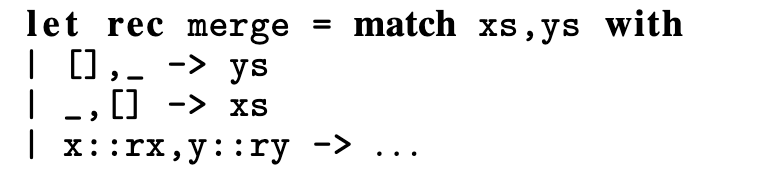
\includegraphics[scale=0.7]{../images/merge.png}
      \Description{Maranget's merge implementation}
      \caption{The skeleton of Maranget's~\tt{merge}}
  \end{figure}

  % He then shows an intermediate representation in his compilation algorithm,
  % the occurrence vector and clause matrix: 

  %~\begin{figure}[H]
  %     \begin{gather*}
  %         \vec{o} = (\tt{xs ys})~\hspace{3em}
  %         P~\rightarrow A = 
  %         \begin{pmatrix}
  %            ~\tt{[]}     &~\tt{\_}     &~\rightarrow~\tt{xs}~\\
  %            ~\tt{\_}     &~\tt{[]}     &~\rightarrow~\tt{ys}~\\
  %            ~\tt{\_::\_} &~\tt{\_::\_} &~\rightarrow~\tt{...} 
  %         \end{pmatrix}
  %     \end{gather*}


  %     \Description{Occurrence vector of names, and clause matrix of matches}
  %     \caption{The occurrence vector and clause matrix are intermediate
  %     representations in Maranget's compilation. I~do not exploit this
  %     representation in my own algorithm, but it helps to understand his final
  %     tree.}
  %~\end{figure}

  The function is compiled to this decision tree: 

  \begin{figure}[H]
      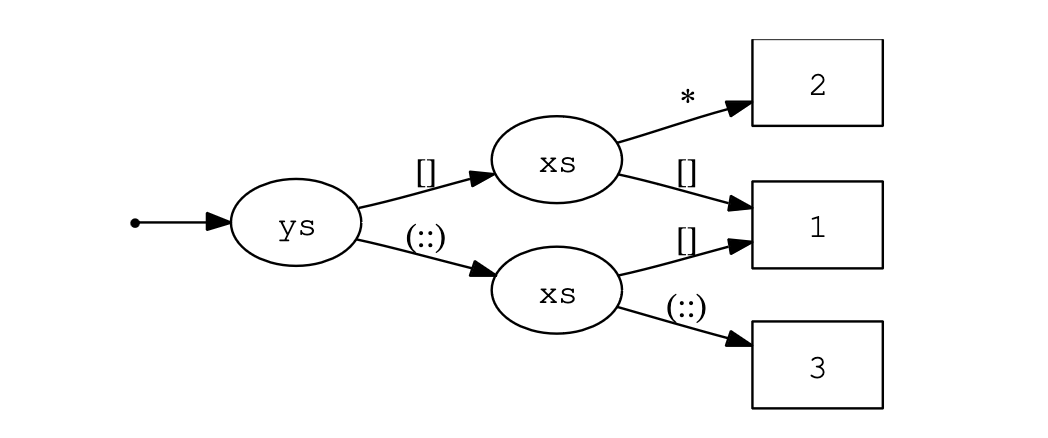
\includegraphics[scale=0.7]{../images/dtree.png}
      \Description{The final decision tree for merge} 
      \caption{The final compiled decision tree for~\tt{merge}, right-to-left}
  \end{figure}

 The decision tree for~\tt{merge}, like the original function, tests values and
 makes decisions. When presented with the values~\tt{xs} and~\tt{ys}, the tree
 first tests ~\tt{xs} against its two known possible forms: the nullary list
 constructor ~\tt{[]}, and an application of the~\it{cons} constructor~\tt{::}.
 If ~\tt{xs} is equal to~\tt{[]}, the tree immediately returns~\tt{ys}. If
 ~\tt{xs} is an application of~\tt{::}, the tree then tests~\tt{ys}
 against~\tt{[]} and~\tt{::}, and it returns a value according to the result of
 the match. Each time the tree goes down a~\tt{::} branch, it extracts the
 arguments of the~\tt{::} for later use: these are~\tt{x}, ~\tt{y},~\tt{xr},
 and~\tt{yr}, which are used in the~\tt{...} branch. This process of extracting
 arguments generalizes to all value constructors with one or more arguments. 

  \begin{figure}
    \begin{center}
    \dcsyntax
    \end{center}
    \Description{The concrete syntax of D.}
    \caption{\D: Concrete syntax}
    \label{fig:dsyntax}
    \end{figure}

  % Here is the decision tree for~\tt{merge} in~\D. 

  %~\begin{figure}[H]
  %   \centering
  %     \it{Like the semantics, this figure is in progress.}
  %     \Description{The decision tree for merge, now in D} 
  %     \caption{The tree for~\tt{merge} in D looks similar to Maranget's.}
  %~\end{figure}

  In~\D, as in Maranget's trees, the~\it{test} node extracts all names from a
  value constructor at once for use in subtrees. The compiler is responsible for
  introducing the fresh names used in~\it{test}. The compiler alpha-renames all
  necessary terms before it translates an~\iffibf to a decision tree to ensure
  all names are unique. 

  In~\D, like in~\VMinus, expressions can~\it{fail}, meaning some of~\D's
  syntactic forms like~\it{try-let} and~\it{cmp} have an extra branch which is
  executed if the examined expression fails. 

    % Includes subsection
    \label{dsemantics}
    \dsemantics


    \subsection{The~\DTran\ algorithm:~\VMinus $\rightarrow$~\D}

    To demonstrate that~\VMinus has a similarly-desirable cost model to pattern
    matching, I~present an algorithm for compiling~\VMinus to a decision tree. I
    choose the decision tree as a target for compilation for the simple reason
    of its appealing cost model. A decision tree can be exponential in size but
    never examines any word of the~\it{scrutinee}---the value being tested---%
    more than once. This property is established by the compilation from~\VMinus
    to \D, which ensuring that no~\it{test} node~\it{T} has any proper ancestor
    \it{T'} such that~\it{T} and~\it{T'} both test the same location in memory.   

    There are a few minor differences in the algorithm I~use and Maranget's: his
    compilation algorithm is more complex than the one in this paper, and
    involves an intermediate representation of occurrence vectors and clause
    matrices which the algorithm I~present does not use. Maranget uses vectors
    and matrices to express multiple simultaneous matches of values to patterns
    as a single match of a vector with a matrix row. This allows him to run a
    \it{specialization} pass that reduces the number of rows in the matrix,
    ultimately leading to smaller trees. Because the trees produced by my
    algorithm still have the linear-in-code-size property, I find them
    acceptable for the current work. 

    The algorithm runs during~\DTran, the transformation from~\VMinus to~\D. Its
    domain, instead of a~\it{case} expression, is~\VMinus's~\iffibf.
    \DTran~propagates a context~\ctx\ which maps each defined name to~\it{known} or
    \it{unknown}. The context is used when determining the form of a guard.
    % in the compilation rules. 
       

    %~\algrenewcommand\algorithmicwhile{\bf{let }}
    %~\algrenewcommand\algorithmicdo{\bf{in }}
    %~\algrenewcommand\algorithmicend{\bf{end}}
    %~\newcommand\alet\algorithmicwhile
    %~\newcommand\ain\algorithmicdo
    %~\newcommand\aend\algorithmicend

    %~\newcommand\branches{\ensuremath{\mathit{branches}}}
    %~\newcommand\mg{\ensuremath{-}}


    When presented with an~\iffibf,~\DTran\~invokes~\Compile with context~\ctx.
    \Compile~first desugars the~\iffibf by expanding choice to multiple~\iffibf
    branches with a desugaring function~\ITran: 
    
    \itran{if\;~\dots~\dbar\; gs_{1};\;~\choiceg{gs_{2}}{gs_{3}};\; gs_{4}~\rightarrow e\;~\dbar~\dots~\;fi}
    
    ==
    
    ${if\;~\dots~\dbar\; gs_{1};\; gs_{2}~\rightarrow e~\;\dbar\; gs_{3};\; gs_{4}~\rightarrow e~\;\dbar~\dots~\;fi}$

    With the desugared~\iffibf,~\Compile\ then repeatedly chooses a guarded
    expression $G$ and applies one of the compilation rules below. The rules are
    applied in a nondeterministic order. 

    The algorithm terminates when it inserts a final~\it{match} node (with rule
    \textsc{Match}).  A~\it{match} node is inserted for a right-hand side expression~\expr when the list of
    guards preceding~\expr is empty or a list of assignments from names to
    unbound names. Termination of~\DTran\~is guaranteed because each recursive
    call passes a list of guarded expressions in which the number of guards is
    strictly smaller, so eventually the algorithm reaches a state in which the
    first unmatched branch is all trivially-satisfied guards.


    If~\Compile\ cannot choose a $g$ of
    one of the valid forms, it halts with an error. This
    can happen when no $g$ is currently solvable in the context, as determined
    by the same algorithm that~\VMinus uses to pick a guard to solve, or when
    the program would be forced to unify incompatible values, such as any value
    with a closure. 

      \subsection{Big-step rules for \Compile}
        \compiler

      \subsection{Reduction Strategies}

      In my implementation, I apply the~\textsc{Test} rule before other rules,
      having found in my experiments that this heuristic leads to the smallest trees. A~%
      risk of inserting a \it{test} node before a \it{let-unless} node is that
      if there are many shared names across branches, a \it{test} node
      will introduce those names in \it{let-unless} nodes in each
      subtree.
      It is possible to insert \it{let-unless} nodes before \it{test}
      nodes, in which case those names will be bound
      only once.  The risk of the \it{let}-first strategy
      is that if there are many names used in only one subtree of a \it{test},
      these names will be introduced to \it{all} branches.  The extra
      bindings may harm
      performance by bloating an environment in an interpreter or thrashing the
      icache if the tree further is compiled to machine code. 

      In the implementation,~\DTran\~first introduces all the names under the
      all existential $\exists$'s to a context which determines if a name is
      \it{known} or~\it{unknown}, applying the~\textsc{Exists} rule is applied
      all at the start. At the start of compilation, each name introduced by
      $\exists$ is~\it{unknown} in a context~\ctx. Since all names in the
      program are unique at this stage, there are no clashes. 

      \subsection{Full Big-step rules for \Compile, with no descriptions}

        The judgement form for compilation is \textsc{Compile}: 

        \showvjudgement{Compile}{\compilebig}

The rules are nondeterministic: the structure of the final result~\expr\ depends
on the order in which rules are applied by the compiler.  

\rawcompiler

    \subsection{Translation from~\VMinus to~\D preserves semantics}
    
    Translating~\iffibf to a decision tree should preserve semantics:
    \begin{conjecture}
      \text{Given a specific but arbitrarily chosen environment~\Rho\; and context~\ctx, when}
      \vmeval[result={\result[1]}]\;and\;\compilebig[iffi=\expr,
      compiled=\expr']\;and\;\vmeval[exp=\expr', result={\result[2]}], then
      {\result[1]} = {\result[2]}. 
    \end{conjecture}
    Proving this conjecture is the subject of future work. 

\end{document}
 
\documentclass[manuscript,screen 12pt, nonacm]{acmart}
\let\Bbbk\relax % Fix for amssymb clash 
\usepackage{vmlmacros}
\AtBeginDocument{%
  \providecommand\BibTeX{{%
    \normalfont B\kern-0.5em{\scshape i\kern-0.25em b}\kern-0.8em\TeX}}}
\usepackage{outlines}
\setlength{\headheight}{14.0pt}
\setlength{\footskip}{13.3pt}
\title{An Alternative to Pattern Matching, Inspired by Verse}

\author{Roger Burtonpatel}
\email{roger.burtonpatel@tufts.edu}
\affiliation{%
\institution{Tufts University}
\streetaddress{419 Boston Ave}
  \city{Medford}
  \state{Massachusetts}
  \country{USA}
  \postcode{02155}
  }
\begin{document}
%~\section{Equations subsume pattern matching with popular extensions}
%~\label{pplustovminus}
%     In my introduction I~stated that~\VMinus can be compiled to a decision tree,
%     and that~\VMinus subsumes pattern matching with popular extensions. Having
%     shown the former, I~now show the latter. I~do so by presenting an algorithm
%     \PtoVTran\ which translates~\PPlus to~\VMinus. 
    
%     % , and proving that the
%     % translation preserves semantics. 

%     \subsection{Domains}

%     I~give the names and domains of the translation functions: 
    
%     \begin{align*}
%         &\PtoVTran:~\PPlus Exp\;~\rightarrow\;~\VMinus Exp~\\
%         &\PTran: Pattern\;~\rightarrow\; Name\;~\rightarrow\; Name\ list\ *\ Guard\ list~\\
%         % &\mathcal{B}: Pattern\; ->\; Name\; Set~\\
%     \end{align*}
    
%     The translation functions~\PtoVTran\ and~\PTran\ are defined case by case: 
    
%     %~\subsection{Binding names}
    
%     %~\begin{align*}
%         %     &\Bindings{x} =~\bracketed{x}~\\ 
%         %     &\Bindings{K} =~\bracketed{}~\\
%         %     &\Bindings{K\; p_{1} {\dots} p_{n}} =~\Bindings{p}~\cup {\dots}~\cup~\Bindings{p_{n}}~\\
%         %     &\Bindings{\porp} =~\Bindings{p_{1}}~\cap~\Bindings{p_{2}}~\\
%         %     &\Bindings{\pcommap} =~\Bindings{p}~\cup~\Bindings{p'}~\\
%         %     &\Bindings{\parrowe} =~\Bindings{p}~\\
%         %     &\Bindings{\whenexpr} =~\bracketed{}
%         %~\end{align*}
        
%         \subsection{Translating Expressions}
        
%         \newcommand\btran[1]{\mathcal{B}[\![#1]\!]}
        
%         \begin{align*}
%             &\ptov[exp=x, result=x]~\\
%             &\ptov[exp={K\;~\expr[1] {\dots}~\expr[n]}, result={K\;~\ptovtran{\expr[1]} {\dots}~\ptovtran{\expr[n]}}]~\\
%             &\ptov[exp={\lambda x.\;~\expr}, result={\lambda x.\;~\ptovtran{\expr}}]~\\
%             &\ptov[exp={\expr[1]\;~\expr[2]}, result={\ptovtran{\expr[1]}\;~\ptovtran{\expr[2]}}]~\\
%             % &\ptov[exp={\tt{case}\;~\expr\;  \emptyseq}, result={{\iffitt{\vexists{x}\; x =~\ptovtran{\expr};\;~\iffitt{}}}}]\;~\rm{, $x$ fresh }   \\
%             &\ptovtran{\tt{case}\;~\expr\;  p_{1}\;~\expr[1]~\vert {\dots}~\vert p_{n}\;~\expr[n]}~\rightsquigarrow~\\
%             &\hspace{2em}~\rm{$\forall i.\; 1~\leq i~\leq n:$}~\\
%             &\hspace{2em}~\tt{if } {\vexists{x}\; x~\tt{ = }~\ptovtran{\expr};}\;~\\
%             &\hspace{2em}~\rm{ let } (\mathit{ns}_{1},~\mathit{gs}_{1}) {\dots} (\mathit{ns}_{i},~\mathit{gs}_{i}) =~\ptran{p_{1}}x\;~\cdot\; {\dots}~\cdot\;~\ptran{p_{i}}x~\rm { in }~\\
%             &\hspace{2em}~\iffitt{\vexists{\mathit{ns}_{1}}\; {\mathit{gs}_{1}}~\rightarrow~\ptovtran{\expr[1]};\;
%                        \square\; {\dots}~\square\;~\vexists {\mathit{ns}_{i}}\; {\mathit{gs}_{i}}~\rightarrow~\ptovtran{\expr[i]}}~\\
%             &\hspace{2em}~\tt{fi}~\\
%             &\hspace{2em}~\rm{, $x$ fresh }
%         \end{align*}
        
%         \subsection{Translating Patterns}
        
%         \begin{align*}
%             &\pattov[pat=y, result={(y, [x = y])}]~\\
%             &\pattov[pat=K, result={([], [x = K])}]~\\
%             &\ptran{K\; p_{1}\; {\dots}\; p_{n}}x~\rightsquigarrow~\\
%             &\hspace{2em}~\rm{$\forall i.\; 1~\leq i~\leq n:$}~\\
%             &\hspace{2em}~\rm{ let } y_{i}~\rm{ be a fresh name, }  \\
%             &\hspace{2em} (\mathit{ns}_{1},~\mathit{gs}_{1}) {\dots} (\mathit{ns}_{i},~\mathit{gs}_{i}) =~\ptran{p_{1}}y_{1}~\cdot {\dots}~\cdot~\ptran{p_{i}}y_{i}~\\
%             &\hspace{2em}~\rm{ in }~\\
%             &\hspace{2em} ({\mathit{ns}_{1}~\cdot {\dots}~\cdot~\mathit{ns}_{i}}~\cdot {y_{1} {\dots} y_{i}}, x = K\; y_{1}\; {\dots}\; y_{i}~\cdot~\;~\mathit{gs}_{1}~\cdot {\dots}~\cdot~\mathit{gs}_{i})~\\
%             &\pattov[pat=\mathit{when}\; e, result={([], [\ptovtran{e}])}]~\\
%             &\pattov[pat=\pcommap, 
%             result={\rm{let } 
%             {(\mathit{ns}_{1},~\mathit{gs}_{1}) =~\ptran{p}x}\; , 
%             {(\mathit{ns}_{2},~\mathit{gs}_{2}) =~\ptran{p'}x}~\rm{ in }
%             (\mathit{ns}_{1}~\cdot~\mathit{ns}_{2},~\mathit{gs}_{1}~\cdot~\mathit{gs}_{2})}]~\\
%             &\pattov[pat=\porp, 
%             result={\rm{let } (\mathit{ns}_{1},~\mathit{gs}_{1}) =~\ptran{p}x\; ,
%             (\mathit{ns}_{2},~\mathit{gs}_{2}) =~\ptran{p'}x~\rm{ in }
%             (\mathit{ns}_{1}~\cdot~\mathit{ns}_{2}, [\mathit{gs}_{1}~\choice~\mathit{gs}_{2}])}]
%         \end{align*}

%     \subsubsection{Significance of the translation}

%     In Section~\ref{extensions}, I~showed how extensions to pattern matching
%     uphold Nice Properties~\ref{p1}~and~\ref{p2}, and how with them, programmers
%     can write more concise code.~\bf{The translation aims to show that if a
%     programmer can code with desirable properties in~\PPlus, they can write code
%     with the same properties in~\VMinus.} Proving this claim formally is a goal
%     for future work. Informally,~\PTran\ does not duplicate code except for
%     introducing new names when translating a constructor-application pattern,
%     and I~believe eliminating this redundancy is possible through a desugaring
%     optimization based off of the laws presented in Section~\ref{ppweird}. 

%     \PtoVTran\ is largely uninteresting, except for the translation from
%     \it{case} to~\iffibf.
        
%     To compile~\it{case} expressions to decision trees as Maranget does,
%     translate~\PPlus to~\D using $(\DTran\; o\;~\PtoVTran)$.
    
%     Finally, I~claim that the translation from~\it{case} expressions to decision
%     trees, $(\DTran\; o\;~\PtoVTran)$, is consistent with Maranget and
%     others~\citep{maranget,scottramsey}. Proving this claim is a good goal for
%     future work; it is not the main focus of this paper. 

    \section{Implementations}

    I~have placed implementations of~\VMinus and~\D at
    \url{https://github.com/rogerburtonpatel/vml}. The implementations are
    complete, from parsers to evaluation to unparsers. In the same repository
    lives the~\tt{dtran} program, which translates from~\VMinus to~\D. With the
    implementations, I~have run testcases to empirically determine the
    correctness of my algorithms, including evaluation of~\VMinus, evaluation
    of~\D, and the translation between the two. I~have determined that the
    translation (empirically) preserves semantics. 


    \section{Related Work}

    This paper builds on Augustsson et al.'s Verse Calculus~\citep{verse} and
    decision trees~\citep{maranget}. Augustsson et al. give the formal rewrite
    semantics for the Verse Calculus; Maranget gives an elegant formalism of
    decision trees and a translation algorithm from patterns to decision trees.
    I~attempted to imitate the behavior of the rewrite semantics of~\VC in the
    big-step semantics of~\VMinus by manually rewriting terms in~\VC and
    creating rules that would imitate the ultimate result of term-rewriting.
    Proving the equivalence between the two semantics is the subject of future
    work. I~chose a big-step semantics because it is the style of semantics I~am
    most comfortable with; writing the formalisms this way helped me write the
    code. Using a rewrite semantics instead would more closely relate~\VMinus
    and~\VC, and is a likely future project. Maranget's formalism was the
    foundation off of which I~built~\D. 
    
    Extensions to pattern matching, and how they appeal to language designers,
    find an excellent example in~\citet{guardproposal}. The authors describe
    pattern guards and transformational patterns (another extension to pattern
    matching), both of which allow a Haskell programmer to write more concise
    code using pattern matching. Or-patterns are documented in the OCaml
    Language Reference Manual~\citep{ocaml}.
    
    \citet{augustsson1985compiling}~ gives a foundation in compiling pattern
    matching. \citet{scottramsey} have a crisp example of a match-compilation
    algorithm (pattern matching to decision trees). Scott and Ramsey's algorithm
    structurally inspired mine, and studying the source code from the paper
    aided my implementation. 
    
    
    \section{Conclusion}

    I~have introduced \VMinus to demonstrate the viability of equations as an
    alternative to pattern matching, and~\D and~\DTran\ to show how both
    languages can be compiled to efficient code. I~have shown with equivalent
    examples how programs written in~\VMinus has the same desirable properties
    as equivalent programs written in~\PPlus, and I~have also shown that
    translating from pattern matching to equations preserves the desirable
    properties. Finally, I~have shown how~\VMinus, like pattern matching, can be
    compiled to efficient code. In doing so, I~have demonstrated that
    programming with equations is a promising alternative to pattern matching. 

    I~have also fully implemented the languages. They exist for use and
    experimentation: they are syntactically simple and have conceptually
    accessible operational semantics. I~hope that programmers will explore and
    develop their own opinions of these languages, which are publically
    available at~\url{https://github.com/rogerburtonpatel/vml}. 

    % Finally, and in particular with~\VMinus, I~hope to provide a stepping
    % stone between pattern matching and equations that a new programmer to
    % Verse will find illuminating. 
    
    % hope to have paved a small
    % segment of the path that the curious programmer or language enthusiast who
    % wishes to better understand Verse will take. Be they transitioning to
    % equations from pattern matching to equations or curious about how those
    % equations might be compilable to decision trees, I~hope they find the
    % languages, and this document, illuminating. 
    
    \section{Discussion and Future Work}        
    \label{futurework}
    
    %~\subsubsection{\VMinus and~\PPlus, side by side}
    % I~compare~\VMinus with~\PPlus as an exercise in comparing equations with
    % pattern matching. They certainly look similar, which hints that~\VMinus
    % might be as expressive as pattern matching with the three extensions. 
    % Proving this claim is the topic of Section~\ref{pplustovminus}. 
    
    % When might a programmer prefer~\VMinus over~\PPlus, or vice versa? After
    % programming in both, I~have come up with three empirical observations: 
    
    %~\begin{enumerate}
    %   \item~\it{The scrutinee:} When there is no obvious single scrutinee,~\VMinus is more succinct.
    %   When there is a scrutinee,~\PPlus is more succinct. 
    %   \item~\it{Binding and decision-making:} Binding and decision-making are
    %   joined in a single construct in~\VMinus:~\tt{=}.~\PPlus needs different
    %   kinds of syntax, like~\tt{<-}, to express different kinds of binding. And
    %   a programmer wanting for~\tt{let} in~\PPlus will never feel this need in
    %   \VMinus:~\tt{=} subsumes that, too. 
    %   \item~\it{Names:} In~\VMinus, names are explicitly introduced. In
    %   practice, this helps prevent a common mistake in pattern matching in which
    %   a programmer attempts to match a value $v$ on an in-scope name $x$,
    %   expecting the match to succeed iff $x$ evaluates to $v$ at runtime, only
    %   to see the match always succeed. 
    %~\end{enumerate}     
    
    %~\rab{How do you feel about examples for each of these points here? This
    % section is very long, but they help drive these points home.}
    
    
    % An example in~\VC illustrates this precise
    % scenario: 
    
    % FIRST PAPER EXAMPLE 
    
    % IMPORTANTLY,~\VMinus REALLY ISN'T A FUNCTIONAL LOGIC PROGRAMMING LANGUAGE ANYMORE. 
    
    %  Doesn't backtrack
    
    %  No multiple results 
    
    %  Doesn't evaluate functions backwards, have top-level patterns like verse, the list goes on 
    
    % If you're well-versed in functional logic programming, may perceive that
    % imposing such restrictions on choice and names effectively strips away
    % much of Verse's essence as a functional logic programming language. With
    % these constraints enforced, there can be no backtracking, multiple
    % results, backward function evaluation, or top-level patterns, among
    % other classic functional logic programming features. But do not fear:
    % our intent is not to recklessly strip Verse of its meticulously crafted
    % core tenets. Instead, our aim is to extract a select few—namely, its
    % equations, existentials, and nondeterministic evaluation order—and
    % juxtapose them with pattern matching.    
    
    
    %~\section{Addressing how~\PPlus handles unusual pattern combinations}
    %~\label{ppweird}
    %     \PPlus admits of strange-looking patterns: consider~\tt{Cons (when true)
    %     zs}. But these should not be alarming, because such syntactic forms reduce
    %     to normal forms by (direct) application of algebraic laws: 
    
    %     \begin{align}
    %       K (\whenexpr)~\;p2\;~\dots &=== K~\;\_~\;p2\;~\dots,~\whenexpr~\\
    %       K (\whenexpr,~\;p2\;)~\;p3\;~\dots  &=== K~\;p2\;~\;p3\;~\dots,~\whenexpr~\\
    %       K (p1\;,~\whenexpr)~\;p3\;~\dots  &=== K~\;p1\;~\;p3\;~\dots,~\whenexpr~\\
    %       K (\whenexpr~\pbar p2\;)~\;p3\;~\dots &=== (K~\;\_~\;p3\;~\dots,~\whenexpr)~\pbar (K~\;p2\;~\;p3\;~\dots)~\\
    %       K (p1~\pbar~\whenexpr)~\;p3\;~\dots &=== (K~\;p2\;~\;p3\;~\dots)~\pbar (K~\;\_~\;p3\;~\dots,~\whenexpr)  \\
    %       \whenexpr~\leftarrow e &===~\;\_ <- e,~\whenexpr
    %     \end{align}   
        
    %     Repeatedly applying these laws until the program reaches a fixed point
    %     normalizes placements of~\it{when}. Laws (2) and (3) work because~\PPlus
    %     has no side effects and the laws assume all names are unique (the compiler
    %     takes care of this), so changing the order in which patterns match has no
    %     effect on semantics.         
    

    \subsection{The design of~\VMinus}
    
    \subsubsection{Forms in \VC and \VMinus}
    
    When designing~\VMinus, I~wanted the language to capture the expressiveness
    of~\VC's equations while retaining a similar decision-making construct to
    pattern matching. In all of pattern matching, the only decision-making
    construct is~\it{case}; all other forms of decision-making like~\it{if}
    desugar to it. In~\VMinus, the only decision-making construct is~\iffibf.
    This differs from~\VC, which features numerous ways to make decisions by
    combining~\bf{one}, \bf{all}, equations, intermediate expressions,
    and~choice. I~did not want multiple results in~\VMinus, so I~eliminated
    anything that looked like~\bf{all}, and I~combined all of the above
    constructs into the singular form~\iffibf. Like~\it{case}, there is only one
    way to use~\iffibf- unlike \bf{one}, equations, intermediate expressions,
    and~choice in~\VC. By restricting all decision-making to \iffibf,
    programmers cannot 'misuse' any of the forms in ways that might lead to
    problematic computations, such as multiple results by returning choice as an
    expression. Furthermore, the way in which programmers use~\iffibf mirrors
    the way they use~\it{case}, as I've shown in the examples. 
    
    \subsubsection{Choice in \VMinus vs. \VC}

    In particular, \VC's choice operator is often the culprit behind both
    backtracking and multiple results, which tempted me to remove choice
    from~\VMinus altogether. However, I~want to harness the expressive potential
    of choice, particularly when paired with~\VC's~\bf{one} keyword. When
    combined with choice, \bf{one} elegantly signifies 'proceed if any branch of
    the choice succeeds.' 
    
    To this end, in~\VMinus, choice is permitted with several modifications:
    
        \begin{enumerate}
        \item Choice may only appear as a condition or 'guard', not as a result
        or the right-hand side of a binding.
        \item If any branch of the choice succeeds, the choice succeeds,
        producing any bindings found in that branch. The program examines the
        branches in a left-to-right order.
        \item The existential $\exists$ may not appear under choice.
        \end{enumerate}
        
        I~introduce one more crucial modification to the~\VC runtime: a name in
        \VMinus is an~\it{expression} rather than a~\it{value}. This alteration,
        coupled with my adjustments to choice, eradicates backtracking. Our
        rationale behind this is straightforward: if an expression returns a
        name, and subsequently, the program imposes a new constraint on that
        name, it may necessitate the reevaluation of the earlier expression—- a
        scenario I~strive to avoid. 

        \subsubsection{Desirable theorems about translations}
        First and foremost, to flesh out the proofs of semantics preservation of
        \PTran\ and~\DTran\ is my top priority. Solid proofs~will strengthen my
        argument that~\VMinus is not only a viable alternative to~\PPlus
        syntactically; it is also formally equivalent. 

        \subsubsection{Desirable theorems about~\VMinus}
        Two theorems would strengthen the viability of~\VMinus, and are
        essential targets for future work:~\bf{Proving~\VMinus~is
        deterministic}, and~\bf{proving the big-step semantics of~\VMinus~is
        consistent with the published semantics of~\VC.} As the authors of the
        Verse paper proved that the rewrite semantics of Verse is
        skew-confluent, I~must prove that big-step semantics of~\VMinus is
        deterministic, despite the nondeterminism of choosing a guard. Second,
        \VMinus~is designed to be Verse-like, and formalizing the relationship
        between the two strengthens~\VMinus's viability as an intermediate
        language between pattern matching and equations. 


        \subsubsection{Exhaustiveness analysis of~\VMinus}
        \label{typingppandvm}

        Exhaustiveness analysis can help restore Nice Property 5: with it, the
        compiler can warn programmers of a missing or extraneous match condition
        in an~\iffibf. Owing to its significantly more flexible structure,
        however,~\iffibf may prove trickier to analyze for missing match
        conditions than \it{case}.

        %~\subsubsection{Type-agnostic decision-making: the $\alpha$}
        %~\label{alphas}

        % The three languages look similar: they each have value constructors and
        % a 'decision-making construct' to deal with constructed data. In~\PPlus, the
        % construct is pattern-matching; in~\VMinus, it is the guarded expression; in~\D,
        % it is the decision tree. 

        % Because of this, it might be possible to make all three languages
        %~\it{higher order} in right-hand sides; that is, to parameterize the
        % expressions that occur~\it{after} all decision-making. Imagine an
        % abstract expression $\alpha$ that appears on the right-hand side of a
        %~\it{case} branch, the right-hand side of a guarded expression, or in a
        %~\it{match} node. The abstract syntax of the new~\it{case},~\iffibf,
        % and decision tree might look like this: 
        %~\begin{center}
        %     \begin{bnf}
        %         $\VMinus_{\alpha}$ :~\VMinus with $\alpha$ ::=
        %         $\mathit{if}\;~\mathit{[}\; g\;~\bracketed{[] g}\;~\mathit{]}\;~\mathit{fi}$ : if-fI~with $\alpha$
        %         ;;
        %         $G_{\alpha}$ : Guarded Expressions with $\alpha$ ::=
        %         $[\vexists{\bracketed{x}}]~\bracketed{g}~\boldsymbol{\rightarrow}\alpha$ : 
        %         ;;
        %         $\PPlus_{\alpha}$ :~\PPlus with $\alpha$::=
        %         $\tt{case}\;~\expr\;~\bracketed{p\;~\ttrightarrow\;~\alpha}$ :~\it{case} expression with $\alpha$ 
        %         ;;
        %         $t_{\alpha}$ : Decision Trees with $\alpha$ ::= 
        %         |~\dots : other forms of tree 
        %         | $\alpha$ : match node 
        %     \end{bnf}
        %~\end{center}

        % Why would one want to do this? Well, recall that~\VMinus had to be
        % stripped of multiple results and other~\VC-like constructs in order to
        % retain its desirable efficiency properties. $\alpha$ lets~\VMinus and
        % the other languages do efficient decision-making without worrying about
        % the form of the result. If the result is a complex multi-value or a
        % computation that involves backtracking, it will be agnostic of the
        % decision-making. $\alpha$ makes right-hand sides polymorphic and
        % abstract, so a programmer could potentially insert expressions from~\VC
        % in their place and know that the decision-making before the $\alpha$
        % will still be efficient. This would allow for fuller interoperability
        % between~\VC and~\VMinus. Section~\ref{vminusandvc} further describes
        % why bridging the gap between the two languages might be a worthwhile
        % exercise. 

        % However, the language designer must take special care to ensure no
        % $\alpha$ finds its way into the decision-making itself, or the whole
        % idea falls apart. I~am developing an implementation that enforces this
        % invariant, and may include it in a future publication. 
        
        % Other alpha material: 
% The decision-making construct that gets us there. Whether
% it's a single value (ML-style) a sequence of values (Verse-style), or
% even something else, the $\alpha$ represents~\it{any} ultimate result of
% "making a decision," and it's the ways in which we make decisions that
% we truly care about examining. By making the return result both
% polymorphic and abstract, we eschew the need to worry about its type and
% compatibility with other results of otherwise-equivalent trees. 

% An expression in core Verse evaluates to produce possibly-empty sequence of
% values. In~\VMinus, values depend on the form of abstract expression $\alpha.$
% If $\alpha$ is a Verse-like expression,~\valpha\ will be a value sequence. If it
% is an ML-like expression, it will be a single value. 
            
%         A guarded expression evaluates to produce a~\bf{result}. A result is either
%         a metavalue~\valpha\ or reject. 
            
%         \[\it{r}\;~\rm{::=}\;~\vartheta\;~\vbar~\;~\reject~\]
            
%         \showvjudgement{Eval-Alpha}{\veval{\alpha}{\valpha}}

% Of note in both~\VMinus and~\D is that the 'decision-making construct'
% is annotated with an $\alpha$. This annotation gives us type flexibility on the
% right-hand side of the~\it{terminating} case for each construct
% (\tt{$\rightarrow$ exp} in~\VMinus and the match node in~\D.) 


        %~\subsubsection{Or-patterns and pattern guards}
        %~\label{pplusindependently}
        %~\PPlus has side conditions, guards, and or-patterns. No major
        % functional language has all three of these extensions. Back
        % Section~\ref{extensions}'s examples, I~had to switch from OCaml to
        % Haskell to use guards, and back to OCaml for or-patterns. The two
        % extensions are mutually exclusive in Haskell, OCaml, Scala,
        % Erlang/Elixir, Rust, F\#, Agda.~\citep{haskell, ocaml, scala, erlang,
        % elixir, rust, fsharp, agda}

        % Why is this the case? In my research, I~have yet to encounter a
        % substantial justification for this. I~have several theories: one,
        % reengineering the Haskell parser to integrate or-patterns into the
        % language may be considered too great an effort; two, the lesser
        % popularity of functional programming in comparison to other paradigms
        % has meant there are not enough voices in any one language's community
        % claiming that theirs needs all known extensions to pattern matching;
        % three, Haskell, the only language with guards, is lazy, and lazy
        % semantics may not operate well with or-patterns. Future work may explore
        % if a lazy semantics of~\PPlus is possible; such a study may answer this
        % question. 

        % \subsubsection{Using~\VMinus to inform programming in Verse}
        % \label{vminusandvc}
        
        % At ICFP last year, Tim Sweeney said that he wanted Verse to be an
        % accessible programming language to write a scalable, collaborative
        % metaverse~\citep{timtalk}. Can~\VMinus be aid in this goal? I~can imagine
        % two ways in which it might:
        
        %~\begin{enumerate}
        %     \item~\VMinus could be  a tool to help ease programmers who are
        %     more familiar with pattern matching into the realm of functional
        %     logic programming with equations. 
        %     \item Programs written in Verse using ideas from~\VMinus might have
        %     a friendlier cost model (depending on the compiler)
        %~\end{enumerate}
        
        % To point~1,~\VMinus sits both syntactically and semantically in between
        %~\PPlus and~\VC, which might help a new programmer to Verse bridge the
        % conceptual gap between pattern matching and equations. Also,~\PtoVTran,
        % the $\PPlus~\rightarrow~\VMinus$ translation, could help a programmer 
        % who wishes to write code using pattern matching see how their ideas 
        % can be expressed in Verse. 

        % To point~2, 
        
        % \DTran\ and the proof that~\DTran\ preserves semantics help show that
        % certain computations that use equations for decision-making can be
        % compiled to efficient code. A future project could be to extend~\VMinus
        % to include~\it{all} of~\VC, and use~\DTran to eliminates as much
        % backtracking at runtime as possible, falling back to the VC's fully
        % general evaluation mechanism only when necessary. My hope is that, using
        % these ideas, both the Verse programmer and language designer might make
        % any discovery that allows them to increase the efficiency of full-Verse
        % programs. 


\end{document}
\documentclass[manuscript,screen, 12pt, nonacm]{acmart}
\let\Bbbk\relax % Fix for amssymb clash 
\usepackage{vmlmacros}
\AtBeginDocument{%
  \providecommand\BibTeX{{%
    \normalfont B\kern-0.5em{\scshape i\kern-0.25em b}\kern-0.8em\TeX}}}
\usepackage{outlines}
\setlength{\headheight}{14.0pt}
\setlength{\footskip}{13.3pt}
\title{An Alternative to Pattern Matching, Inspired by Verse}

\author{Roger Burtonpatel}
\email{roger.burtonpatel@tufts.edu}
\affiliation{%
\institution{Tufts University}
\streetaddress{419 Boston Ave}
  \city{Medford}
  \state{Massachusetts}
  \country{USA}
  \postcode{02155}
  }
\bibliographystyle{ACM-Reference-Format}
\usepackage[utf8]{inputenc}

\begin{document}

\section{Acknowledgements}

This thesis would not have been possible without the infinitely generous time
and support of my advisors, Norman Ramsey and Milod Kazerounian. Norman's
offhand comment of “I~wonder if Verse's equations subsume pattern matching” was
the entire basis of this work, and his generosity in agreeing to advise a full
thesis to answer his question will always be profoundly appreciated. During the
academic year, Norman provided me with materials on both the technical story and
on how to write about it well. He gave me regular feedback and has helped
improve my research skills, my technical writing, and my understanding of
programming languages in general tremendously. I~especially appreciate how he
has guided me in-person at the end of my undergrad when his book~\citep{bpc} got
me started down the path of PL at the beginning of it. Finally, Norman is also
fantastically fun to pair program with. 

From the beginning, Milod provided me with encouraging mentorship that kept
me enthusiastic and determined to complete the project. He was exceptionally
patient as I~gave him whirlwind tour after whirlwind tour of the changing
codebase and problems, and he kept me grounded in the problems at hand. He 
sent me helpful examples of his research to aid me in my proofs, and gave me
some particularly encouraging words towards the end of the project that I~
will not soon forget. 

My undergraduate advisor, Mark Sheldon, has always been both supportive and
kind. I~have enjoyed many long talks in his office, and I~am deeply grateful
that he is on my committee. 

Alva Couch was the advisor of my original thesis idea, which was to compile
programming languages with music. Ultimately, we decided that I~should pursue
this project instead, and I~am grateful to him for his mentorship in that moment
and onwards. 

My family---my mother, Jennifer Burton, my father, Aniruddh Patel, and my
sister, Lilia Burtonpatel, have all given me support, encouragement, and
(arguably most importantly) food. My gratitude for them is immeasurable. 

My gratitude towards my friends is also without limit. In particular, and in
no order, Liam Strand, Annika Tanner, Max Stein, Cecelia Crumlish, and
Charlie Bohnsack all showed specific interest in the work and encouraged me
as I~moved forward. Rachael Clawson was subjected to much rubber-ducking,
and endured valiantly. Aliénor Rice and Marie Kazibwe were as steadfast
thesis buddies as I~could ever hope for. Jasper Geer, my PL partner in
crime, was always one of my favorite people to talk to about my thesis. His
pursuits in research inspire mine. 

Skylar Gilfeather, my unbelievable friend. Yours is support that goes
beyond words; care, food, silent and spoken friendship, late night rides to
anywhere, laughs and tears are some that can try to capture it. I~am so, so
grateful for how ceaselessly you've encouraged me on this journey. Every one
of your friends is lucky to have you in their life, and I~am blessed that 
you are such a core part of mine. 

Anna Quirós, I~am writing these words as you sleep behind me. Your support
and love have been immeasurable. I~will always be grateful to you for this
year~\it{increíble}. I~could not have smiled through it all without you. 

Thank you all. 

%\section{References}
\bibliography{sources}

\renewcommand\thesection{\Alph{section}}
\setcounter{section}{0}
% \section{Proofs}
% \begin{outline}
% \1~\bf{Proof: Translation from~\VMinus to~\D\ preserves semantics }
% \begin{proof}
%   In progress. 
% \end{proof}
% \1~\bf{Proof: Translation from~\PPlus\ to~\VMinus preserves semantics }
% \begin{proof}
%   In progress. 
% \end{proof}
% %~\1~\bf{Proof: Translation from~\VMinus to Verse preserves semantics}
% \end{outline}


\section{Is~\VMinus\ a true subset of~\VC?}
\VMinus\ certainly appears to relate to~\VC\ semantically. If they are formally
related, \VMinus may inform programming in \VC, which could help new Verse
programmers learn the language if they are familiar with more traditional
decision-making constructs like \iffibf. By starting with \VMinus, they could
move from subset to full set as they learn the full Verse language. 

Translating \iffibf and choice in~\VMinus to~\bf{one} and choice in~\VC\ is
likely a sufficient embedding. Formalizing this translation and, more
importantly, proving that my semantics of~\VMinus are consistent with Augutsson
et al.'s \VC\ is an excellent goal for future work. 

\section{Formal Definitions of all languages}
\label{languagedefs}

\begin{table}[H]
  \utable
  \caption{Abstract Syntax of~\VMinus and~\D. Forms in black are present in both
              languages, forms in~\red{red} are specific to~\VMinus, and forms
              in~\blue{blue} are specific to~\D.}
  \label{fig:unilang2}
\end{table}

\subsection{Rules (Big-step Operational Semantics) for~\U, shared by~\VMinus and~\D}
\label{usemantics1}
\usemantics 
\subsection{Rules (Big-step Operational Semantics) specific to~\VMinus}
\label{vmsemantics2}
\vmsemantics
\label{dsemantics2}
\dsemantics

\subsection{Full Big-step rules for \Compile, with no descriptions}


\showvjudgement{Compile}{\compilebig}

\subsection{Rules (Big-step Translation) for compiling \iffibf}

These rules in a nondeterministic order by the compiler. 

\[
\inferrule*[Left=\textsc{ (Exists) }]
    {\compilebig[ctxext={\bracketed{x_1 \mapsto unknown}}, gexps={\GsgsGs{\vexists{\dots x_{n}}\; \gs \rightarrow \expr'}}]}
    {\compilebig[gexps={\GsgsGs{\vexists{x_{1} \dots x_{n}}\; \gs \rightarrow \expr'}}]}
\]

\[
\inferrule*[Left=\textsc{ (Fail) }]
    {\compilebig[gexps=\GsGs]}
    {\compile[guard={\fail}]}
\]


\[
\inferrule*[Left=\textsc{ (Match) }]
    {\ }
    {\compilebig[gexps={\GsgsGs{}}]}
\]

\[
\inferrule*[Left=\textsc{ (Test) }]
    {\rho(x) = known
    \\\\
    \compilebig[ctxext={ + \overline{\bracketed{y_{i} \mapsto known}}}, 
             iffi=\subst{\expr}{K_{i}\; {\ybar[i]}}{x}, compiled={\expr[i]}]
    \\\\
    \tbar = \sum_{i} K_{i}\; \ybar[i] \Rightarrow \expr[i]
    \\\\
    \expr[0] = \subst{\expr}{K_{0}}{x} \and K_{0} \text{ does not appear in } e
    }
    {\compile[eas={\expr \text{ as }}, guard={x = K\; \expr[1] \dots \expr[n]},
    compiled={test(x, \tbar, \expr[0])}]}
\]

\[
\inferrule*[Left=\textsc{ (Elim-Vcon) }]
    {
    \compilebig[gexps=\GsGs]
    \\\\
    \expr[lhs] \text{ does not have the form } K\; \expr'[1] \dots \expr'[n]
    }
    {\compile[guard={\expr[lhs] = K\; \expr[1] \dots \expr[n]}]}
\]

\[
\inferrule*[Right=\textsc{ (Expand-Vcon) }]
    {
    \compile[guard={{\expr[1]}' = \expr[1];\; \dots;\; {\expr[n]}' = \expr[n]}]
    }
    {\compile[guard={K\; {\expr[1]}' \dots {\expr[n]}' = K\; \expr[1] \dots \expr[n]}]}
\]

\[
\inferrule*[Right=\textsc{ (Let-Unless) }]
    {\rho(x) = unknown \and \knownj[exp=\expr']
    \\\\
    \compilebig[ctxext={\bracketed{x \mapsto known}}, iffi=\subst{\expr}{x}{\expr'}, compiled=\dt_{1}]
    \\\\
    \dt_{2} = \subst{\expr}{\fail}{\expr'}
    }
    {\compile[eas={\expr \text{ as }}, guard={x = e}, 
              compiled={let\; x = \expr'\; in \; \dt_{1}\; unless\; \fail\; \Rightarrow\; \dt_{2}}]}
\]


\[
\inferrule*[Right=\textsc{ (Let-If) }]
    {\rho(x) = known \and \knownj[exp=\expr'] 
    \\\\
    \dt_{1} = \subst{\expr}{x}{\expr'}
    \\\\
    \compilebig[ctxext={\bracketed{y \mapsto known}}, iffi=\subst{\subst{\expr}{\fail}{x = \expr'}}{y}{\expr'}, compiled=\dt_{2}] \and y \text{ fresh}
    \\\\
    \dt_{3} = \subst{\expr}{\fail}{\expr'}
    \\\\
    \dt_{if} = {if\; x = y\; then\; \dt_{1}\; else\; \dt_{2}}
    }
    {\compile[eas={\expr \text{ as }}, guard={y = e}, 
              compiled={let\; x = \expr'\; in \;{\dt_{if}}\; unless\; \fail\; \Rightarrow\; \dt_{3}}]}
\]


%~\begin{figure}
%~\begin{center}
%     \begin{bnf}
%     $P$ :~\textsf{Programs} ::=
%     $\bracketed{d}$ : definition
%     ;;
%     $d$ :~\textsf{Definitions} ::=
%     | $\tt{val}\; x\;~\tt{=}\;~\expr$ : bind name to expression
%     ;;
%     $\expr$ :~\textsf{Expressions} ::=
%     | $v$ : literal values 
%     | $x, y, z$ : names
%     | $\tt{if}\; [\; G\;~\bracketed{\tt{[]}\; G}\;]\;~\tt{fi}$ : if-fi 
%     | $K~\bracketed{\expr}$ : value constructor application 
%     | $\expr[1]\;~\expr[2]$ : function application 
%     | $\ttbackslash x\tt{.}\;~\expr$ : lambda declaration 
%     ;;
%     $G$ :~\textsf{Guarded Expressions} ::=  
%     $[\tt{E }{\bracketed{x}}{\tt{.}}]~\bracketed{g}~\;\ttrightarrow\;~\expr$ : names, guards, and body
%     ;;
%     $g$ :~\textsf{Guards} ::=  
%     | $\expr$ : intermediate expression 
%     | $x~\;\tt{=}\;~\expr$ : equation 
%     | $ g~\bracketed{\tt{;} g}~\;~\pbar~\; g~\bracketed{\tt{;} g}$ : choice 
%     ;;
%     $\v$ : Values ::= $K\bracketed{\v}$ : value constructor application 
%     | $\ttbackslash x\tt{.}\;~\expr$ : lambda value
%     \end{bnf}
%~\end{center}
%~\Description{The concrete syntax of PPlus.}
%     \caption{\VMinus: Concrete syntax}
%     \label{fig:vmsyntax}
%     \end{figure}

%~\begin{figure}
%     \begin{center}
%     \begin{bnf}
%     $P$ :~\textsf{Programs} ::=
%     $\bracketed{d}$ : definition
%     ;;
%     $d$ :~\textsf{Definitions} ::=
%     | $\tt{val}\; x\;~\tt{=}\;~\expr$ : bind name to expression
%     ;;
%     $\expr$ : Expressions ::= 
%     | $v$ : literal values 
%     | $x, y, z$ : names
%     | $K\bracketed{\expr}$ : value constructor application 
%     | $\ttbackslash x\tt{.}\;~\expr$ : lambda declaration  
%     | $\expr[1]\;~\expr[2]$ : function application 
%     | $\tt{case}\;~\expr\;~\bracketed{p\;~\ttrightarrow\;~\expr}$ : case expression 
%     |~\ttbraced{$\expr$}
%     ;;
%     $p$ :~\textsf{Patterns} ::= $p_{1}\pbar p_{2}$ : or-pattern
%     | $p~\tt{,} p'$ : pattern guard 
%     | $p\;~\tt{<-}\;~\expr$ : pattern from explicit expression  
%     | $x$ : name 
%     | $\tt{\_}$ : wildcard 
%     | $K\;~\bracketed{p}$ : value constructor application 
%     | $\tt{when}\;~\expr$
%     |~\ttbraced{$p$}
%     ;;
%     $\v$ : Values ::= $K\bracketed{\v}$ : value constructor application 
%     | $\ttbackslash x\tt{.}\;~\expr$ : lambda value 
%     ;;
%     $K$ :~\textsf{Value Constructors} ::=
%     | $\tt{true}\;~\vert\;~\tt{false}$ : booleans
%     | $\tt{A-Z}x$ : name beginning with capital letter
%     % | $[\tt{-}\vert\tt{+}](\tt{0}-\tt{9})+$ : signed integer literal 
%     \end{bnf}
%     \end{center}
%     \Description{The concrete syntax of PPlus.}
%     \caption{\PPlus: Concrete syntax}
%     \end{figure}

\end{document}


\end{document}
\endinput
%%
